\documentclass[12pt,oneside]{book}

\usepackage[dvips,letterpaper,margin=0.75in,bottom=0.75in]{geometry}
\usepackage{cite}
\usepackage{slashed}
\usepackage{graphicx}
\usepackage{amsmath}
\usepackage{enumitem}
\usepackage{amsthm}
\usepackage{braket}
\usepackage{listings}
\theoremstyle{definition}
\usepackage{pythonhighlight}

\usepackage[american,fulldiode]{circuitikz}
\tikzset{component/.style={draw,thick,circle,fill=white,minimum size =0.75cm,inner sep=0pt}}

\newcounter{plot}[chapter]
\setcounter{plot}{0}

\newcommand{\plot}{
\stepcounter{plot}
\noindent
{\bf $\bigtriangleup$ Jupyter Notebook Exercise \thechapter.\theplot:}
}


\newcounter{pencil}[chapter]
\setcounter{pencil}{0}

\newcommand{\pencil}{
\stepcounter{pencil}
\noindent
{\bf $\bigtriangleup$ Pencil and Paper Exercise \thechapter.\theplot:}
}


%\newtheorem{pencil}{Pencil Problem}[chapter]
%\newtheorem{plot}{Jupyter Notebook}[chapter]


\lstnewenvironment{algorithm}[1][] %defines the algorithm listing environment
{   
    \lstset{ %this is the stype
        mathescape=true,
        frame=tB,
        numbers=left, 
        numberstyle=\tiny,
        basicstyle=\scriptsize, 
        keywordstyle=\color{black}\bfseries\em,
        keywords={,input, output, return, datatype, function, in, if, else, foreach, while, begin, end, repeat, print, calculate,} %add the keywords you want, or load a language as Rubens explains in his comment above.
        numbers=left,
        xleftmargin=.04\textwidth,
        #1 % this is to add specific settings to an usage of this environment (for instnce, the caption and referable label)
    }
}
{}


\begin{document}
\ctikzset{bipoles/thickness=1}
\ctikzset{bipoles/length=.6cm}

\title{Physics 40 Lab Manual}
\author{Michael Mulhearn}
\maketitle

\tableofcontents

\chapter{Installation of Scientific Python}

\section{Introduction}

In this lab, you will install the software which we will be using in
phy40. This is an assignment, and will be graded.  You should submit a
text file containing a log of all the steps you took to install the
software on your computer.  Make this log as specific as possible, an
entry might be:
\begin{verbatim}
Downloaded windows installer from:
 https://repo.anaconda.com/miniconda/Miniconda3-latest-Windows-x86_64.exe
\end{verbatim}  
Keeping this log will also make it easier for you to get help if you
have problems.

If you run into problems, do some research on a web search tool
(Google, for example) to become better informed and to see if you can
overcome the problem on your own before asking for help.  This is an
important technique in getting help with technical problems that will
serve you well even outside of this class.  You will find it more easy
to get useful technical help, from the sort of people most capable of
offering it, when it is clear from your question that you are informed
and have already tried all of the obvious things.  If you are still
stuck after trying to solve the problem for yourself, then contact
your TA or instructor with specific technical details about what is
failing, and include your installation log.

If you do find a problem with these instructions or manage to overcome
a technical problem yourself, make sure to note it in your log and
inform your TA, in case it is helpful for other students.

\section{Installing Miniconda3}

We will be using Miniconda3 based on Python 3.7 for data analysis
using Jupyter notebooks.  Miniconda is a lightweight package which we
can use to install all of the remaining analysis software we will need
in a consistent manner across all different operating systems.

Determine which OS type and version you have on the desktop or laptop
computer that you will be using for your coursework.  The software
here will work under Windows, Linux, or macOS.  It should also work on
all Chromebooks released since 2019, and some earlier Chromebooks.
You should also check whether you have a 32-bit or 64-bit OS (you can
find instructions for how to determine this for your particular OS
version with a Google search.)  Most desktop or laptop computers built
in the last ten years are 64-bit.

If you are using Linux or macOS, then from within a terminal type:
\begin{lstlisting}{language=csh}
 echo $SHELL
\end{lstlisting}
to determine the shell you are using (typically "bash" these days).
Record all of this information in your installation log file.

Once you have determined your OS type and version, follow the
instructions below approprate to your operating system.

\subsection{Installing under Windows}

If you have already installed a version of conda (e.g. Anaconda or
Miniconda) then you do not need to re-install it.  Instead, find the
the Anaconda Prompt in the Application menu and run it.

If you need to install Miniconda3, then download and run the
appropriate installer from:
\begin{verbatim}
https://docs.conda.io/en/latest/miniconda.html#
\end{verbatim}
If prompted, you should choose to:
\begin{itemize}
 \item Accept the license / terms of use.
 \item Install for just the current user, not all users.
\end{itemize}
 Once installed, check that you can run the "Anaconda Prompt". From
the prompt, check that you can run:
\begin{lstlisting}{language=csh}
  conda --version
\end{lstlisting}
and note the output in your installation log.  Then proceed to
Section~\ref{sec:env}.

\subsection{Installing on a Chromebook}

You will need to activate Linux on your Chromebook, according to the instructions here:

\begin{verbatim}
https://www.codecademy.com/articles/programming-locally-on-chromebook
\end{verbatim}

Then follow the insturctions for installing under Linux.  If your
Chromebook predates 2019 and does not support Linux, contact your
instructor for alternative arrangements.

\subsection{Installing Miniconda3 under Linux or macOS}

If you believe you already already have a version of conda installed
(such as miniconda or ananconda) , check by running
\begin{lstlisting}{language=csh}
   conda --version
\end{lstlisting}
If you see something like:
\begin{lstlisting}{language=csh}
  conda 4.9.2
\end{lstlisting}
as output (even if the version is different) then you do indeed already have conda
installed, with the base environment activated, and you can skip ahead to
Section~\ref{sec:env}.  If instead you get a message like:
\begin{lstlisting}{language=csh}
   conda: command not found
\end{lstlisting}
then the easiest solution is to simply proceed with these instructions.

To install Miniconda, download the appropriate installer for your OS
here:
\begin{verbatim}
  https://docs.conda.io/en/latest/miniconda.html\#
\end{verbatim}
For macOS, you can choose between a "package" or "bash" version. I
find it easier to follow the bash version, but the package version
will work too. I recommend you make the following choices if prompted:
\begin{itemize}
\item Accept the license / terms of use.
\item Do not install for all users, but just one the current user.
\item Do allow the installer to issue ``conda init''.
\end{itemize}
During the installation, take note of the install location in your log.

After installation with these settings, conda will automatically
activate the ``base'' conda environment.  If this annoys you, as it
does me, or interferes with other software you are using, you can turn
off this agressive behavior with:
\begin{lstlisting}{language=csh}
   conda config --set auto_activate_base false
\end{lstlisting}

Confirm that you have successfully installed conda by typing
\begin{lstlisting}{language=csh}
   conda --version
\end{lstlisting}
Record the output in your installation log, and proceed to Section~\ref{sec:env}.

\section{Installing the Physics 40 Conda Environment}
\label{sec:env}

Make sure your conda is fully up to date with:
\begin{lstlisting}{language=csh}
  conda update conda
\end{lstlisting}
Then follow the prompts, e.g. selecting "y" as needed to update any out-of-date packages.

We'll be using a conda environment specifically for phy40 to avoid
conflicts with any other projects on your computer, and to ensure that
we all have the same software installed.  To create our environment:
\begin{lstlisting}{language=csh}
  conda create -n phy40 python=3.9 numpy scipy matplotlib ipython jupyter
\end{lstlisting}
  
\section{Starting a Jupyter notebook}

This course will make extensive use of the Jupyter Notebook interface
to Scientific Python, which is well suited to academic work (including
independent research) because it combines code with output in
digestable chunks.  Even when the end product is a polished peice of
software, much of the initial code development can be done in the interactive
session that Jupyter Notebooks provide.  

\begin{figure}[htbp]
\begin{center}
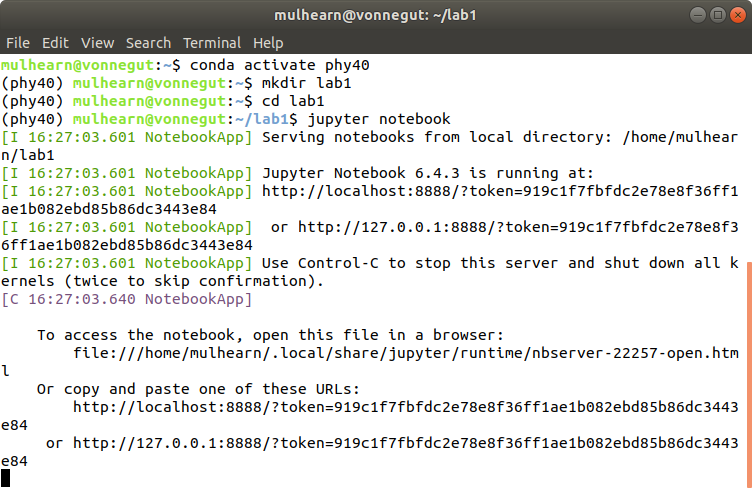
\includegraphics[width=0.65\textwidth]{figs/install/jupyter_startup.png} 
\caption{Example starting Jupyter Notebook from the Linux command line.  In Windows, you will need to open the Anaconda Prompt instead of a terminal.}
\label{fig:jupyterstartup}
\end{center}
\end{figure}

\begin{figure}[htbp]
\begin{center}
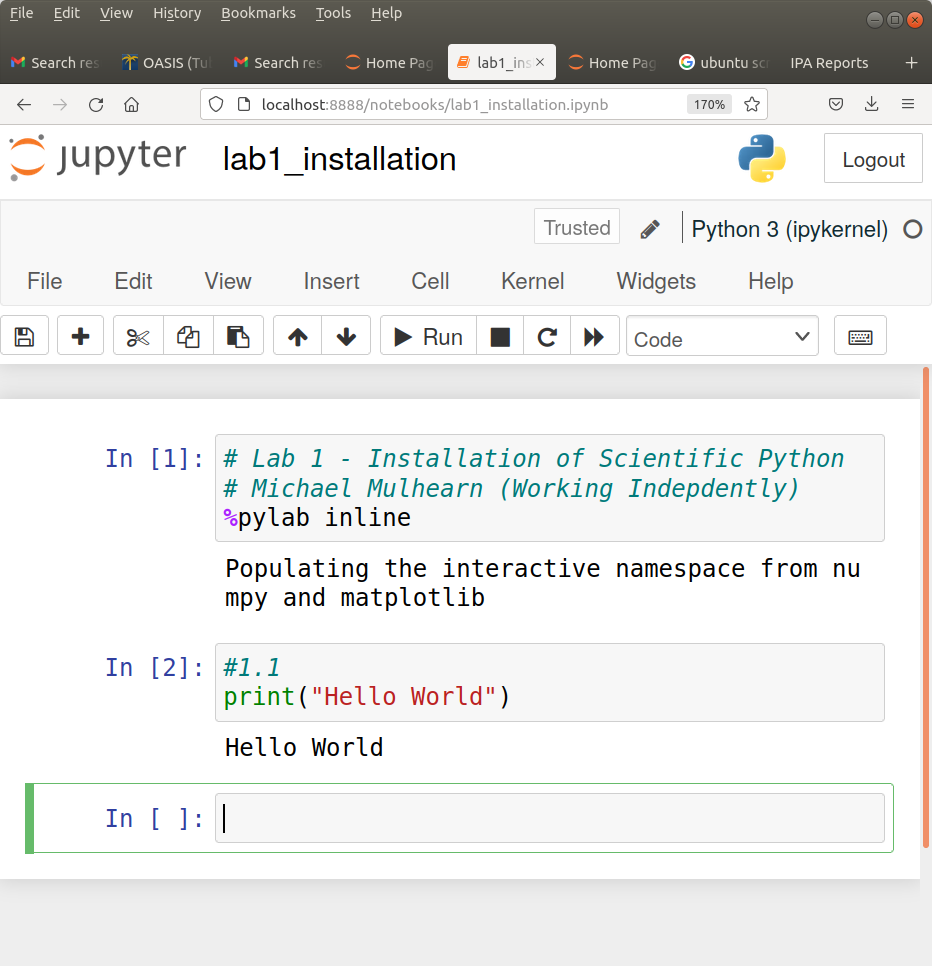
\includegraphics[width=0.65\textwidth]{figs/install/jupyter_window.png} 
\caption{The Hello World example Jupyter Notebook.}
\label{fig:jupyterwindow}
\end{center}
\end{figure}

\begin{figure}[htbp]
\begin{center}
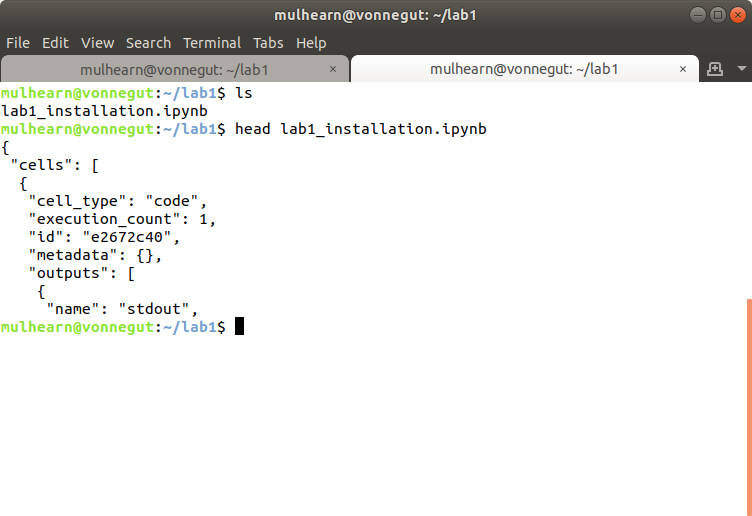
\includegraphics[width=0.65\textwidth]{figs/install/jupyter_saved.png} 
\caption{Example showing the saved Jupyter notebook.  Notice that notebook file (ipynb) is not human readable on its own: it requires the Jupyter software to render it in a human readable form.}
\label{fig:jupytersaved}
\end{center}
\end{figure}

To activate the phy40 environment type:
\begin{lstlisting}{language=csh}
  conda activate phy40
\end{lstlisting}
When you are done with Phy 40 for the day you can deactivate this
environment (later) with:
\begin{lstlisting}
  conda deactivate
\end{lstlisting}
Launch jupyter notebook with:
\begin{lstlisting}
  jupyter notebook
\end{lstlisting}
This should start the Jupyter Notebook server and open a client in your web browser.
An example starting a Jupyter Notebook from Linux is shown in Fig.~\ref{fig:jupyterstartup}.

You should create one Jupyter Notebook per lab assignment, by choosing
the New (Python 3) option in your client.  Change the name of your
notebook to something that clearly identifies the lab.  Start each lab
with comments (starting with ``\#'' symbol) indicating the title of
the lab, then your name followed by your lab partners.  See the first
cell of Fig.~\ref{fig:jupyterwindow} for an example.  This first cell
is also a good place to issue the ipython ``magic function'':
\begin{verbatim}
%pylab inline
\end{verbatim}
which will setup the notebook for inline plots and load the numpy and matplotlib libraries for you.

Each assignment will consist of a number of steps, clearly numbered like this one, your first step:\\

\plot Print ``hello world'' using the python print command.\\

\noindent
To keep your notebook clear, label cells (such as this one) with a
comment for the assignment step number, as in the second cell of
Fig.~\ref{fig:jupyterwindow}.  You only need to label one cell if the
assignment is fullfilled across several cells.

Jupyter Notebook checkpoints your work automatically.  You should be
able to see your notebook saved in the working directory where you
started, as in Fig.~\ref{fig:jupytersaved}.  Notice that while the
notebook file is ASCII text, it is not a human readable format.  The
Jupyter software is needed to render the notebook in a human readable
way.  To make your grader's life easier, you will be submitting PDF
versions of your notebook, once all of the tasks are completed and the
output is visible.  There are several ways to make a PDF file from
your notebook, but the most reliable is to use the ``Print Preview''
option to view the notebook as a PDF file within your browser, then
use the print feature of your browser to print the page as a PDF file.
Try this now, and make sure you can create a legible PDF file, but do
not submit it to the course site, as you still have more to do.
Always keep your python notebook file (ipynb) even after you submit
the assignment.  If you have problems, you can reproduce a PDF file
from the notebook file, but it is tedious to reproduce your notebook
from PDF.  If you have problems producing the PDF file, you can submit
the ``ipynb'' file as a temporary work-around, but work with your TA
to sort out the problem as quickly as possible.

\section{Submitting your assignment}

Before submitting, take some time to clean up your assignments to
remove anything superfluous and place the exercises in the correct
order.  You can also add comments as needed to make your work clear.
You can use the Cell $\to$ All Output $\to$ Clear and Cell $\to$ Run
All commands to make sure that all your output is up to date with the
cell source.

When you are satisfied with your work, print the PDF file as described
earlier and submit it to the course website.











\chapter{Binary Numbers}

\section{Introduction}

At the heart of numerical analysis, naturally, you will find numbers.
In this lab, we will explore the basic data types in Python, with
particular emphasis on the computer representation of integers and
real numbers.  All modern programming languages do an admirable job of
hiding the limitations of the computer representations of these
mathematical concepts.  In this chapter, we will deliberately explore
their limitations.

\section{Preparation}

This lab will rely on the material from Section 1.2.2 of the
Scientific Python Lecture notes.\\

\plot Enter the following code into a cell and check the output:
\begin{python}
a = 121
print(type(a))
print(a)
\end{python}
Next, in the same cell, add a line at the end setting $a$ to a real value, \pyth{a = 1.34}, and
print the type and value again.  Check the output.  Next, set $a$ to Boolean value,
\pyth{a = False}, and print the type and value yet again. \\

In many languages, such as C and C++, variables are strictly typed:
you would have to decide at the start whether you want $a$ to be of
integer, float, or boolean type, and then you would not be able to
change to a different type later.  Python variables are references to
objects, which means they only point to memory locations that contain
objects with all of the data and functionality associated with that
object.  When you write $a = 121$ it is interpreted as ``set variable
$a$ to point to a location in memory that contains a class of type
integer with the value 121''.\\

\plot Enter the following code into a cell and check the output:
\begin{python}
a = 12
b = a
b = 5
print(a)
print(b)
\end{python}  
Why is the output ``12, 5'' instead of ``5, 5''?  When you write
\pyth{b = a}, the variable $b$ points to the same Integer class that
$a$ points to.  So when you write ``b = 5'' why doesn't the value of
$a$ change as well?  This code snippet shows that it does not.  The
reason is that Integers are {\em immutable} objects in python... their
values cannot be changed.  So when you write \pyth{b = 5} it is
interpreted as ``variable b points to a (new) Integer with value 5.''
The variable a continues to point to the Integer with value 12.  The
``is'' operator used like this:
\begin{python}
  print(a is b)
\end{python}
tells you if $a$ references the same object as $b$.  Add to compiles
of this line to your snippet in order to clarify the situation.  One
call should return True and the other False.\\

\plot If I set a variable $a$ to an integer value and I set $b$ to
the same integer value, do $a$ and $b$ refer to the same object, or to
two different objects with the same value?  Write a snippet of code
(three lines) to find out.\\

In this lab, it will be convenient to know how to calculate the absolute value of a number, which you can do with the python \pyth{abs} function:
\begin{python}
a = -1.5
b = abs(a)
print(b)
\end{python}


\section{Binary Representation of Integers}

Computer hardware is based on digital logic: the electrical voltage of
a signal is either high or low, which correspond to a mathematical
zero or one.  A digital clock is used to ensure that signals are only
sampled at particular times, when they are guaranteed not to be in
transition from a zero to one or vice versa.  The Arithmetic-Logic
Unit (ALU) uses digital logic gates (such as AND or OR) to perform
calculations.  For example, it is possible to build an adder that uses
only NAND gates.

Because digital signals have only two states (zero and one), the most
natural way to represet numbers in a computer is using the base two,
which we call binary.  In the familiar base ten, we have ten digits
(from 0 to 9) and the place value increases by a factor of 10 with
each digit moving toward the left.  In binary, we have only two digits
(0 and 1) and the place value increase by factors of two.  A single
digit in binary is referred to as a ``bit''.  You add columns quickly
when counting in binary: zero(0), one(1), two(10), three(11),
four(100), five(101), and so on.  For efficient operations, computers
often group eight bits together to form a byte.  Digital values are
therefore commonly represented in hexidecimal (base 16) where two
digits of hexidecimal describes one byte.  See Table~\ref{tbl:binary},
which you can produce for yourself in Python like this:
\begin{python}
print("dec: hex: bin:")
for d in range(16):
    print("{0:<2d}   0x{0:01x}   0b{0:04b}".format(d))
\end{python}
It is conventional to preprend binary numbers with ``0b'' and
hexadecimal with ``0x'' otherwise we wouldn't know whether a ``10''
represents ten, sixteen, or two!  Notice that the largest number that
can be written with $n$ bits is $2^n-1$.

\begin{table}
\begin{center}
  \caption{The numbers 0 to 15 in decimal, hexadecimal, and binary.}
  \label{tbl:binary}
\begin{tabular}{|lll|lll|}
\hline
dec: & hex: & bin: & dec: & hex: & bin: \\
\hline
0  & 0x0  & 0b0000 & 8  & 0x8  & 0b1000 \\ 
1  & 0x1  & 0b0001 & 9  & 0x9  & 0b1001 \\
2  & 0x2  & 0b0010 & 10 & 0xa  & 0b1010 \\
3  & 0x3  & 0b0011 & 11 & 0xb  & 0b1011 \\
4  & 0x4  & 0b0100 & 12 & 0xc  & 0b1100 \\ 
5  & 0x5  & 0b0101 & 13 & 0xd  & 0b1101 \\
6  & 0x6  & 0b0110 & 14 & 0xe  & 0b1110 \\
7  & 0x7  & 0b0111 & 15 & 0xf  & 0b1111 \\
\hline
\end{tabular}
\end{center}
\end{table}

The mathematical notion of an integer can be naturally implemented by
computer hardware.  Although integers are represented in binary in the
hardware, modern compilers and languages generally print them to
screen as decimal by default.  One caveat is that computers do not
have an unlimited number of bits.  Many computer languages use 64-bit
integers, which means that only the integer values from 0 to
18446744073709551615 can be represented:
\begin{python}
x = 2**64-1
print(x) 
\end{python}
For signed integers, one bit is used to indicate the sign (positive or
negative) and so a 64-bit signed integer can represent integer values
from -9223372036854775808 to 9223372036854775807.  As long as an
integer value is within the range covered by the integer type, the
integer value can be perfectly represented.

Python uses arbitrary sized integers: it simply adds more bits as
needed to represent any number.  For an extremely large number, you
will eventually reach practical limitations on the amount of memory
and processing time available in the computer, which will limit how
large of an integer can be calculated.\\

\plot See for yourself just how huge integers can be in python by entering:
\begin{python}
x = 2**8000
print(x)
\end{python}
and checking the output.\\

\plot Print the integer 64206 in decimal, hexadecimal, and binary.  Hint: just reuse the carefully formatted print statement from the example above.\\

\plot Suppose you are tasked with rewriting the firmware for a 
distant satelite which has just lost one line from an eight-bit
digital communications bus due to radiation damage.  You now have only
seven working bits!  What is the maximum sized unsigned integer which
you could write on this degraded seven-bit bus?  What range of signed
integers could you write? \\

% FIXME:  in future years, use the paper and pencil macro here:
\plot This is a paper and pencil exercise.  You can do it on paper and
pencil and submit a scanned PDF, or you can just record you steps as
comments in a jupyter notebook cell.  Let's consider a four-bit signed
integer, so zero is 0000 and one is 0001.  Suppose the upper bit is
reserved for sign, so 1XXX is a negative number.  An obvious choice
for representing -1 would be 1001, but there is a better choice.
Consider that:
\begin{displaymath}
(-1) + 1 = 0  
\end{displaymath}
Well, if we simply ignore the last carry bit (5th bit):
\begin{displaymath}
1111 + 1 = 10000 = 0000  
\end{displaymath}
So if we define 1111 as -1, we can treat addition with negative numbers exactly the same as adding ordinary numbers.  Find the representation for -2 such that
\begin{displaymath}
-2 + 2 = 10000 = 0000
\end{displaymath}
then show that:
\begin{displaymath}
-1 + -1 = -2. 
\end{displaymath}
Python does not use this trick, but many other languages do.\\

\section{Binary Representation of Real Numbers}

Representing real numbers presents much more of challenge.  There are
an uncountably infinite number of real numbers between any two
distinct rational numbers, but a computer has only finite memory and
therefore a finite number of states.  It is impossible for computers
to exactly represent every real number.  Instead, computers represent
real numbers with an approximate floating point representation much
like we use for scientific notation,
\begin{displaymath}
x = m \times B^n
\end{displaymath}
where the significand $m$ is a real number with a finite number of
significant figures and the exponent $n$ is an integer.  The base $B$
is ten for scientific notation but typically two in a floating point
representation.  The exponent $n$ is typically chosen so that there is
only one digit before the decimal point in the base $B$, e.g. $3.173
\times 10^{-8}$ for scientific notation.

The limited precision of the discriminant can lead to challenges when
using floating point numbers.  The floating point precision is
specified by the parameter $\epsilon$ (epsilon) which is the
difference between one and the next highest number larger than one
that can be represented.  For scientific notation with four
significant digits, $\epsilon=0.001$, because we cannot represent
anything between $1.000 \times 10^0$ and $1.001 \times 10^0$ with only
four significant figures. \\

\plot Determine the Python floating point $\epsilon$ by running
\begin{python}
import sys
print(sys.float_info.epsilon)
\end{python}

\vskip 0.25cm
\begin{plot} \end{plot} Determine the Python floating point $\epsilon$ for yourself by running:
\begin{python}
eps = 1.0
while eps + 1 > 1:
    eps = eps / 2
eps = eps * 2
print(eps)
\end{python}
Here the while loop continues running the indented code until the
condition $\epsilon+1=\epsilon$ is met.

\newpage
\vskip 0.25cm
\plot Python uses the IEEE 754 double-precision
floating-point format.  This format uses 64-bits overall, with 52 bits
reserved for the significant.  The standard uses a clever trick to
save one bit, by requiring that the leading bit of the significant $m$ is
one, and defining 53 signficant figures using 52 bits:
\begin{displaymath}
m = 1.m_1 m_2 m_3 ... m_{52}
\end{displaymath}
Here each $m_i$ represents an individual bit (0 or 1).  Predict the
parameter $\epsilon$ and compare with the above. \\


\plot It seems like $\epsilon$ should be small enough to simply ignore
it in most cases, but in fact it shows up quite clearly if you apply
strict equality to floating point quanties.  To see the problem, run
this code, checking if $\sin(\pi)$ is zero:
\begin{python}
x = np.sin(np.pi)
print(x)
print(x==0)
\end{python}
The strict equality condition $x==0$ is not met because of limited
floating point precision.  Instead of strict equality, check that $x$
is near zero with a condition like:
\begin{displaymath}
|x| < 10 \epsilon
\end{displaymath}
where $\epsilon$ is the machine precision and the factor of 10 is a
conservative factor to allow for round-off errors that might be a bit
larger than the best possible precision $\epsilon$.  Add such a
condition to the code above and show that this looser definition of
equality now holds.  In general, when using approximations (like
floating point numbers) you can only check things to within the
accuracy of the approximation!\\

\plot Here is another case where floating point precision joins the
chat uninvited:
\begin{python}
x = 0.1
y = x+x+x
print(y == 0.3)
\end{python}
Devise an alternative to \pyth{y==0.3} that properly accounts for
floating point precision.\\

\plot Personally, I prefer my zero's to look like zero.  When floating
point limitations are making them look non-zero, I like to clean then
up with rounding, like this:
\begin{python}
x = np.sin(2*np.pi)
print(x)
x = np.around(x,15)
print(x)
\end{python}
Yeck! What is $-0$??!!  IEEE 754 defines two zeros $-0$ and $0$.  $-0$
is used to indicate that $0$ was reached by rounding a negative
number.  This is so that $1/-0$ can be interpreted as $-\infty$ and
$1/0$ as $+\infty$.  If you just want to make this go away, add ``+0'':
\begin{python}
x = np.around(x,15)+0
\end{python}
Show that this works.\\

\plot Consider the following code:
\begin{python}
a = 5;
b = 1.2343E-17;
sum = 0
sum += 5;
for i in range(1000000):
    sum = sum + b
print(sum)
\end{python}
Is there any problem here?  If there is, fix it by changing only the {\em order} of the lines of code.


\section{Other Data Types}

Integers and floating point numbers are the real work horses of
computational physics.  We'll add numpy arrays in a future lab.  This
section will briefly introduce the remaining types.

Python includes strings as a basic type:
\begin{python}
s = "hello world"
s = s + " (it's been a strange few years)"
print(s)
print(type(s))
print(s[6],s[4],s[6])
print(type(s[0]))
\end{python}
Strings are {\em immutable} objects that contain textual data.  If you
have used other languages, you might expect \pyth{s[0]} to be a
``character'' but in Python it is a string of length one.  There is no
built-in character type.

Python includes complex numbers as a basic type:
\begin{python}
  z = 1 + 2j
  print(type(z))
  print(z.real)
  print(z.imag)
  print(z.conjugate())
\end{python}
This is our first example of an object oriented programming (OOP)
class interface.  To compute the complex conjugate of $z$, an ordinary
function would need to be passed $z$ as an argument, or else it would
not know which complex value to use for the computation.  But
\pyth{z.conjugate()} is a {\em method} of the class complex.  The
method is tied to the instance of complex number $z$ by the ``.'' and
has access to all of the data it needs from $z$.  Similarly,
the \pyth{real} and \pyth{imag} are member data of class complex: they
are the integers that contain the real and imaginary parts of $z$.
Objects play a central role in Python, but in a refeshingly
understated and reserved manner.  It is enough for now to understand
that \pyth{z.conjugate()} is much like a function that already has $z$
as a parameter, and \pyth{z.imag} and \pyth{r.real} are just ways to
access the data contained in $z$.\\

\plot Define a complex number with value of $1+i$ and multiply it by
it's complex conjugate.  Show that the resulting complex number has
zero for it's imaginary part.\\

Python provides Lists as a native container of python objects.  We'll
make much more use of numpy arrays, which are better suited to
numerical analysis, but Python Lists occassionally play a role for various
bookkeeping tasks:
\begin{python}
L = ["hello", 1, 2, 3+2j, 3.45, "green"]
print(L[0])
print(L[1])
print(L[5])
L[0] = "goodbye"
print(L)
\end{python}
Here the List $L$ contains a variety of (admittedly rather useless)
objects.  These objects can be referred to individually by their
index.  One place where lists really shine is in looping over a
custom list of values:
\begin{python}
for i in [1,5,10,50,100]:
    print(i)
\end{python}

\vskip 0.25cm
\plot Run the following code:
\begin{python}
  a = [1,2,3,4,5]
  b = a
  b[0] = 3
  print(a[0])
  print(a is b)
\end{python}
(Spits out coffee) ``What the???!!''  Lists are {\em mutable} which makes
them fundamentally different from {\em immutable} integers.  Here
we assign $b$ to point to the same object as $a$ (a list) and then
change an entry in that list.  Even after the change, $a$ and $b$
point to the same object.  This is only possible because the list
object is mutable. \\

\plot It's good to read the documentation, but it's a useful skill to
figure things out for yourself too!  Without looking up the
documentation, write a snippet of code to determine for yourself if
complex numbers are mutable (like lists) or immutable (like integers).
We are able to change just a part of a list (like \pyth{a[0]=3}).  But can we change part of a complex number (like \pyth{z.real}).  Try it and find out!

(It's OK if your code throws an error here, but you can also comment
it out if you are the sort of person that can't possibly leave it
alone)\\
















\chapter{Sequences and Series}

\section{Introduction}

In this lab, we will apply for loops to study sequences and series.
If you already have programming experience, you can complete a
challenge problem in lieu of some of the other problems: see the final
problem for the details.

\section{Preparation}

This lab will rely on the material from Sections 1.2.1 to 1.2.4 of the
Scientific Python Lecture notes.  Most of the problems can be
completed using a simple functions containg a single for loop, such as
in this function:
\begin{python}
  def loop(n):
    for i in range(n):
        print(i)
\end{python}
To run the code in the function, you call the function, usually in a different cell:
\begin{python}
loop(5)
\end{python}

\vskip 0.25cm
\plot Create a new function:
\begin{python}
def mult(a,n):
   # your code here ...
\end{python}
that prints the first n multiples of a.  For example \pyth{mult(3,4)} should output:
\begin{python}
3
6
9
12
\end{python}
In future problems, we'll describe this output simply as 3, 6, 9, 12.
We won't be picky about whitespace unless we discuss it explicitly.
One way to complete this is to use the three arguments of
\pyth{range(start,stop,step)}.

\section{Fibonacci Sequence}

The Fibonacci numbers are a sequence of numbers satisfying the
recursion relationship:
\begin{displaymath}
F_{n+2} = F_{n} + F_{n+1}
\end{displaymath}
with $F_0=0$ and $F_1=1$.  The sequence is:
\begin{displaymath}
0, 1, 1, 2, 3, 5, 8, 13, 21, 34, \ldots
\end{displaymath}
This sequence can be generated numerically by an algorithm such as this one:
\begin{algorithm}
fa := 0 # set fa to 0
fb := 1 # set fb to 1
repeat n times: 
   fc := fa + fb
   print fc to screen
   fa := fb
   fb := fc
\end{algorithm}
Note that this is not python syntax.  What is the importance of the
last two lines?  Would the algorithm work if we exchanged their order?\\

\plot Use the algorithm described above to implement a new function
\pyth{fib(n)} which prints the next $n$ Fibbonacci numbers after the
initial 0 and 1.\\

\section{Arithmetic Series}

The finite arithmetic series
\begin{displaymath}
  S_n = \sum_{k=0}^{n} (a + kd) = a + (a+d) + (a+2d) + \ldots + (a+nd)
\end{displaymath}
sums to the average of the first and last terms times the number of terms:
\begin{equation} \label{eqn:arithsum}
S_n = (n+1)\frac{a + (a+nd)}{2}
\end{equation}
We will assume $a=d=1$ and calculate this finite series numerically using the following function:
\begin{python}
def arith(n):
    sum = 0
    for j in range(1,n+1):
        sum = sum + j
        #print("j: ", j, "\t sum: ", sum)
    return sum    
\end{python}
Type in this function and see how it works by uncommenting the print
statement (delete the \# symbol that starts a comment) and calling it
as \pyth{arith(5)}.  The use of print statements in a loop like this
or at each stage of a calculation is a simple, effective and classic
debugging technique.  You test your code with the print statements
included, keeping n small so you don't fill your whole screen with
output. Once your code is working, you comment out the unneeded print
statements so that the interpreter ignores them and you no longer
see the unneeded output.  Why not just delete them?  You can, but
experience shows that if you do, you will need the line again shortly!\\

\plot Obtain the sum of the first $n$ terms of arithmetic series with
\pyth{sum = arith(n)} for three different values of $n$.  Each time,
show that sum returned by the function matches the expected sum.

\section{Geometric Series}
\label{sec:geom}

The geometric series
\begin{displaymath}
  \sum_{k=0}^{\infty} a r^k = a + ar + ar^2 + ar^3 + \ldots
\end{displaymath}
converges for $|r| < 1$ to:
\begin{equation} \label{eqn:geomsum}
  \frac{a}{1-r}.
\end{equation}
We will demonstrate this numerically.\\

\plot Implement a function \pyth{geom(a,r,n)} which calculates sum of the first $n$ terms of the geometric series with $k$th term $a r^k$.  Show that it agrees with Eqn.~\ref{eqn:geomsum} for $a=2$, $r=0.5$  $n=100$.
\\

\plot Call you geometric series function again for $a=3$, $r=0.8$ and $n=100$.  Compare with the expected output calculate within python and with pencil and paper.  Do they agree exactly?  If not, do they agree within the floating point precision?
\\

\plot Now compare your calculated sum with Eqn.~\ref{eqn:geomsum} for $a=1$, $r=-0.9$  $n=100$.  How is the agreement?  Increase $n$ and see what happens.  Why do you suppose this series is slower to converge?\\

\section{Refinements}

There are a few refinements you can make to your code.  Don't change
your working code from previous examples!  Instead, copy the previous
version to a new cell and make your refinements there.  You don't even
need to change the name of the function, Python will happily overwrite
the old function implementation when it reaches the cell with the new
version.  Make these code improvements:\\

\plot (Optional) Improve your Fibbonacci function so that prints the
first $n$ numbers including the initital two numbers ``0'' and ``1''.
Make sure it works properly for $n=0$, $n=1$, $n=2$, and so on.\\

\plot (Optional) Extend the Arithmetic series function to include
parameters $a$ and $d$.  Show that it works.\\

\section{Fibonacci Integer Right Triangles}

Starting with the number 5, every second Fibonacci number is the
length of the hypotenuse of a right triangle with integer sides.  The
first two are:
\begin{displaymath}
5^2 = 3^2 + 4^2  
\end{displaymath}
and 
\begin{displaymath}
13^2 = 5^2 + 12^2.  
\end{displaymath}
Furthermore, from the second triangle onward, the middle side is the sum of the lengths of the sides of the previous triangle, for example:
\begin{displaymath}
12 = 3 + 4 + 5.  
\end{displaymath}

\vskip 0.25cm
\plot (Optional Challenge) Use numerical methods to
explicitly verify these properties for the first $n$ Fibonacci integer
right triangles.\\

If you would prefer, you may submit the Optional Challenge problem plus the
problems from Section~\ref{sec:geom} to complete the assignment.


\chapter{The Quadratic Equation and Prime Numbers}

\section{Introduction}

In this lab, we will make more extensive use of conditional statements
to implement algorithms which solve the quadratic equation, identify
prime numbers, and add fractions.  An optional challenge problem,
The Lucky Number of Euler, explores how the quadratic equation can
generate prime numbers.

\section{Preparation}

This lab will rely on the material from Sections 1.2.1 to 1.2.4 of the
Scientific Python Lecture notes.  We'll now be making frequent use of
conditional statements:
\begin{python}
def compare(a,b):
    if (a==b):
        print("a equals b")
    elif (a<b):
        print ("a is less than b")
    else:
        print ("a is greater than b")
\end{python}
Notice that Python uses \pyth{==} for comparison.  You will get a
syntax error if you use \pyth{a=b} instead.

We'll also use of the modulo operator $\%$ extensively.  The modulo
operation $a\%b$ returns the remainder from the integer division
$a/b$.
\begin{python}
# is b a factor of a?
def isfactor(a,b):
    if (a%b == 0):
        return True;
    return False
\end{python}
Why does \pyth{a%b == 0} mean that b is a factor of a?\\

\newpage
\vskip 0.25cm
\plot Consider this verbose code snippet:
\begin{python}
for i in range(100):
    print("on index ", i)
\end{python}
Which prints the current index on every iteration.  Use the modulo
operator to modify the code so that it only prints the index every 10
iterations.  This is a classic trick!\\

We will also be using while loops, which repeat a block of code until a condition is met:
\begin{python}
count=0
while(count<10):
    print(count)
    count = count+1
\end{python}

\section{Quadratic Formula}

The Quadratic equation:
\begin{displaymath}
  ax^2 + bx + c = 0
\end{displaymath}
has solutions which are given by the quadratic formula
\begin{equation} \label{eqn:quad}
x = \frac{-b \pm \sqrt{b^2 - 4ac}}{2a}
\end{equation}
The number of unique real solutions depends on the quantity in the
square root, which is called the discriminant:
\begin{displaymath}
b^2-4ac
\end{displaymath}
If this is positive there are two real solutions, it it is one there
is one real solution, and if it is negative there are no real
solutions.

The solution to the quadratic equation can be calculate as follows:
\vskip -0.25cm
\noindent
\begin{algorithm}
  D := b^2 - 4ac
  if (D<0): 
     print no solutions
  if (D>0):
     calculate both solutions from quadratic formula
     print both solution
  if (D=0):
     calculate the single solution from quadratic 
     print single solution
\end{algorithm}
\vskip 0.25cm
Since $D$ is calculated from parameters $a$, $b$, and $c$ which might
be floating point, we need to take some care to evaluate the condition
that \pyth{D==0} within the precision of the floating point operation.

A test case with one real solution is:
\begin{displaymath}
(x-1)(x-1)= x^2 -2x + 1.
\end{displaymath}
A test case with two real solution is:
\begin{displaymath}
(x-1)(x+1)= x^2 - 1.
\end{displaymath}
A test case with zero real solutions is:
\begin{displaymath}
(x-i)(x+i)= x^2 + 1.
\end{displaymath}

\vskip 0.25cm
\plot Implement a function \pyth{quad(a,b,c)} which reports the solutions to the quadratic equation and verify it with the test cases shown.\\

\plot Calculate three more test cases with integer solutions and use them to test your function more thoroughly. \\

\plot A particular tricky test case is a=.1 b=.3 c =0.225 which should
have only one real solution.  Test you function against this test case. \\

\section{Prime Numbers}

A prime number is a number that has two and only two factors: itself and one.
One is not prime, but two is.
We can determine if a number $a$ is prime as follows:
\vskip 0.25cm
\begin{algorithm}
  if (a<2):
     return false
  i := 2
  while ($i \leq \sqrt{a}$):   
     if (a%i=0):
        return false
     i := i + 1
  return true
\end{algorithm}
\vskip 0.25cm
Why is there no need to check for factors larger than $\sqrt{a}$?\\

\plot Implement a function \pyth{isprime(a)} which returns \pyth{True}
if the integer $a$ is prime and \pyth{False} if not.\\

Suppose that next we want to find the first $n$ prime numbers greater
than or equal to a number $A$.  We can simply check if $A$, $A+1$,
$A+2$, and so on are prime until we find the first $n$.  But we do not
know how many numbers we will have to check before finding $n$ that
are prime.  This is a case for a \pyth{while} loop.\\

\plot Find the first $n$ prime numbers greater than $A$ using a while
loop and your \pyth{isprime} function. Test it for $n=10$ and $A=0$,
then for $A=1000000000$.  Try that with paper and pencil!\\

Notice how we broke this problem of finding primes into two parts:
determining whether or not a number is prime or not, then testing and
counting prime numbers.  We thoroughly tested the first part before
using it in the second.  This is an essential approach to solving
computational problems: break complicated tasks down into smaller
tasks which can be tested separately.\\

\plot Implement a function which computes the fraction
\begin{displaymath}
\frac{n}{d} = \frac{a}{b} + \frac{c}{d}
\end{displaymath}
from integer inputs $a$,$b$,$c$ and $d$ and returns integers $n$ and
$d$.  Returning $n>d$ is allowed, but $n/d$ should be a simplified
fraction with a greatest common factor of one.  You can return two
integers as a Tuple, like this:
\begin{python}
  # function which	adds fractions
  def addfrac(a,b,c,d):
     n=d=0
     #your code...
     return n, d
     
  # calling function:
  n,d =addfrac(1,2,1,3)
  print("{0}/{1}".format(n,d))
\end{python}
For full credit, you must factorize (see what I did there?) this
problem into two parts: your \pyth{addfrac} funtion should call a
second function that does one well defined task.
\section{The Lucky Number of Euler}

Euler discovered that the formula:
\begin{displaymath}
k^2 + k + 41
\end{displaymath}
produces prime numbers for $0 \leq k \leq 39$.  Perhaps you can beat Euler at his own game!

Consider quadratics of the form:
\begin{displaymath}
k^2 + ak + b
\end{displaymath}
For each integer value of $a$ and $b$, there is a maximum number $n$ such that the quadratic formula produces prime numbers for $0 \leq k < n$\\

\plot Find the the values of $a$ and $b$ which produce the largest number of prime numbers.  Restrict yourself to $|a| \leq 1000$ and $|b| \leq 1000$.



\end{document}


\chapter{Introduction to Plotting}

\section{Introduction}
This exercise will introduce calculations and plotting techniques using
numpy arrays within Scientific Python.

\section{Plotting discrete data and continuous functions}

\begin{figure}[htbp]
\begin{center}
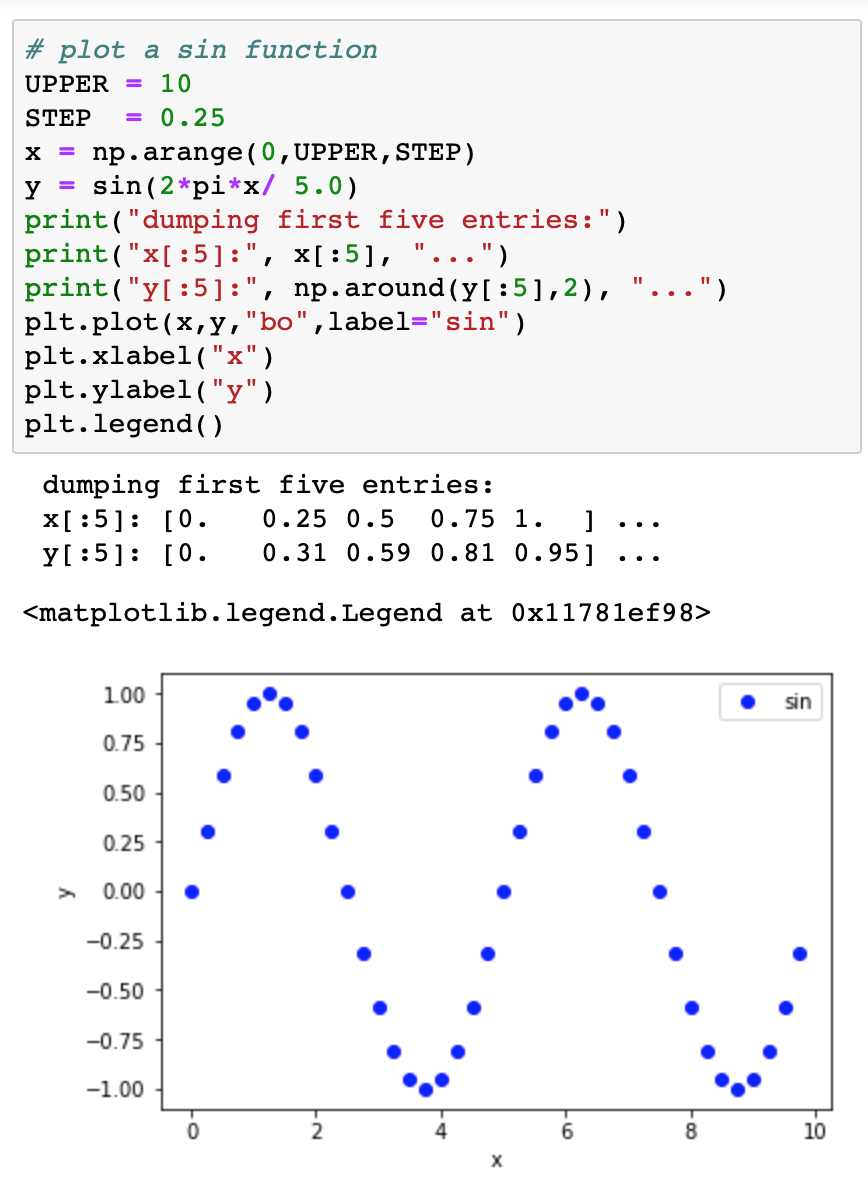
\includegraphics[width=0.65\textwidth]{figs//plotting/plotting.png} 
\caption{Circuit for verifying Ohm's law as a (a) circuit diagram, and (b) implemented using your lab equipment.}
\label{fig:plotsin}
\end{center}
\end{figure}

Consider the Jupyter notebook example in Fig.~\ref{fig:plotsin} which
plots a sine function sampled at discrete values.  Note the following
key features, which you will use repeatedly today and in future labs:
\begin{itemize}
\item Use of global variables {\tt UPPER} and {\tt STEP} at the top of
  the snippet, allowing for easy adjustment of parameters that affect
  the plot.
\item Use of {\tt np.arange} to define an array of x values.
\item Creation of the array y, defined by $y = \sin(2\pi x / 5)$ for each value of x.  One of the great joys of using numpy is the ability to avoid getting bogged down with explicit for loops.
\item Use of slicing techniques {\tt x[:5]} to show only the first five entries for debugging.  
\item Plotting the arrays of $x$ and $y$ values with {\tt plt.plot}  using the {\tt "bo"} option for blue circles.
\item Defining appropriate axis labels with {\tt plt.xlabel} and {\tt plt.xlabel}. 
\item Creation of a legend using the {\tt label} option to {\tt plt.plot} and the {plot.legend()} command.
\end{itemize}
Notice that even in this simple example, I've added some intermediate
feedback from my code in the form of the screen dumps of the first few
values of $x$ and $y$.  It's a common pitfall to try and rush ahead to
the final product when programming.  But it is much faster and
reliable to break your task into small steps, and establish feedback
at each small step.  To plot a continuous function with Scientific
Python, you will still use discrete data but:

\begin{itemize}
 \item Use much finer binning of the $x$-axis variable to draw a smooth curve. 
 \item Use the line option {\tt "-"} or dashed line {\tt "--"} instead of points with {\tt "o"}. 
\end{itemize} 

\noindent
{\bf Plot 1:}  Plot the quadratic function $y = x^2$ with the following requirements:
\begin{itemize}
 \item Plot in the range $x = [0,20)$.
 \item Plot discrete samples with a step size of $2$ using blue circles.
 \item On the same axis, plot the corresponding smooth function using a red solid line.
 \item Add appropriate axis labels. 
 \item Add a legend for the ``discrete'' and the ``smooth''  function.
\end{itemize}

\section{Multivariate analysis using boolean masks}
\begin{figure}[htbp]
\begin{center}
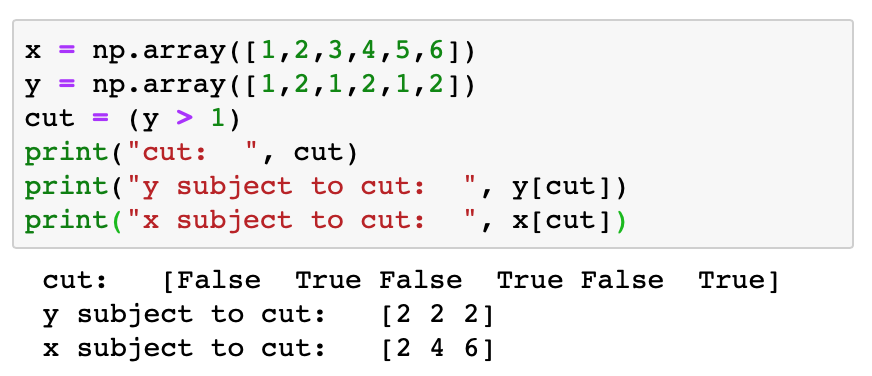
\includegraphics[width=0.65\textwidth]{figs//plotting/booleanmasks.png} 
\caption{Using boolean masks to cut on variable $y$.}
\label{fig:booleanmasks}
\end{center}
\end{figure}

A powerful technique in Scientific Python for performing analysis involving multiple variables uses boolean masks as shown in Fig.~\ref{fig:booleanmasks}.  In the example:
\begin{itemize}
\item Two numpy arrays $x$ and $y$ {\tt of the same length} are defined to contain the collected data.
\item The cut defined by $y > 1$ is a boolean array of the same length as $x$ and $y$ which is true at indices where the condition is met and false where it is not.
\item The subset of the entire $y$ array defined by {\tt y[cut]} consists only of those entries of $y$ for which the condition $y>1$ is met.
\item The subset of the entire $x$ array defined by {\tt x[cut]} consists only of those entries of $x$ for which the condition $y>1$ is met for the corresponding y value.
\end{itemize}
The last item shows the real power of this technique, one can look at one variable subject to constraints on another variable.

\begin{table}
\caption{Sample data for a voltage measurement subject to high frequency noise.}
\label{tbl:hfnoiseeg}
\begin{center}
\begin{tabular}{lll}
$t~(\rm s)$ & $v~(\rm V)$ & $n$ \\
0.4  & 0.25  &  2.8 \\
1.1  & 2.37  &  7.3 \\
1.4  & 1.69  &  9.7 \\
1.9  & 0.93  &  1.3 \\
2.5  & -1.0  &  6.2 \\
3.0  & 0.95  &  4.8 \\
3.4  & 1.22  &  6.9 \\
4.1  & 0.54  &  4.0 \\
4.4  & 0.37  &  1.9 \\
4.8  & 0.13  &  4.0 \\
5.5  & -2.04  &  9.5 \\
6.2  & -2.06  &  8.7 \\
6.5  & -0.81  &  2.3 \\
7.0  & -0.95  &  5.3 \\
7.5  & 0.98  &  9.7 \\
7.9  & 0.27  &  8.3 \\
8.5  & -0.81  &  0.1 \\
9.0  & -0.59  &  5.1 \\
9.4  & -0.37  &  4.4 \\
9.9  & 0.56  &  9.9 \\
\end{tabular}
\end{center}
\end{table}

Next consider the sample data in Table~\ref{tbl:hfnoiseeg} which comes from experimental measurements of a voltage level $v$ at discrete times $t$.  The measurement is subject to a high-frequency noise monitoring by the variable $n$.  The noise is only present for $n > 6.0$.  A straightforward way to load this data into scientific python is by defining numpy arrays for each variable as follows:
\begin{verbatim}
t = np.array([0.4, 1.1, 1.4, 1.9, 2.5, 3.0, 3.4, 4.1, 4.4, 4.8, 
                     5.5, 6.2, 6.5, 7.0, 7.5, 7.9, 8.5, 9.0, 9.4, 9.9])
v = np.array([ 0.25, 2.37, 1.69, 0.93, -1.0, 0.95, 1.22,   
                      0.54, 0.37, 0.13, -2.04, -2.06, -0.81, -0.95,  
                      0.98, 0.27, -0.81, -0.59, -0.37, 0.56])
n = np.array([2.8, 7.3, 9.7, 1.3, 6.2, 4.8, 6.9, 4.0, 1.9, 4.0,  
                      9.5, 8.7, 2.3, 5.3, 9.7, 8.3, 0.1, 5.1, 4.4, 9.9])
\end{verbatim}

\noindent
{\bf Plot 2} Prepare a plot of the sample data subject to the following:
\begin{itemize}
 \item Plot the voltage as a function of time as discrete data using red points.
 \item Define the boolean array {\tt keep} based on the noise reducing condition $n<=6.0$.
 \item Plot the voltage as a function of time, subject to the noise reducing condition using blue points.
 \item Plot the function $\sin(2 \pi x / 10)$ as a smooth function.
 \item Add appropriate axis labels.
 \item Add a legend for ``raw'' data with no cut, ``clean'' data with noise removed, and your continuous ``sin'' function.   
\end{itemize}
Your plot will reveal a clear sine function in the discrete data (after noise removal) consistent with the continuous function.  






\chapter{Differentiation and Projectile Motion}

\section{Introduction}

In this lab we will apply numerical differentiation to elementary
functions.  We'll apply the Euler method to compute the trajectory of
a projectile, and compare our results with the analytic solution.
We'll also show that our numerical technique easily accommodates air
resistance, a problem that has no analytic solution using elementary
functions.

\section{Preparation}

Our code is going to get complicated enough that we will need to pay
some attention to variable scope, as illustrated here:
\begin{python}
i=1
j=2
k=3
def f(i,j):
    print(i,j,k)
f(i,j)
f(j,i)
\end{python}
Try to predict the output of this snippet before running it.  The
first three lines define integers $i$,$j$, and $k$. These have global
scope, which means they can be accessed from anywhere.  The function
\pyth{f(i,j)} has parameters $i$ and $j$ which have a scope limited to
the function $f$.  Even though they have the same name as the global
variables $i$ and $j$, they are independent quantities.  Within the
function $f$ the variable $i$ is the first parameter, and $j$ is the
second parameter.  Because they have the same name, the global
variables $i$ and $j$ are {\em shadowed} by the local parameters $i$
and $j$.  The global variable $k$ is not shadowed.

In this lab, we will also be passing a function as an argument to another
function, as in this simple example:
\begin{python}
def show(f):
    print(f(2))
    print(f(3))    
    
def f(i):
    return i**2

def g(i):
    return i**3

show(f)
show(g)    
\end{python}
Here the \pyth{show} function takes another function \pyth{f} as an
argument.  Within the show function, the function \pyth{f} is called
using paranthesis just like any other function, as in \pyth{f(2)} We
define two additional functions, \pyth{f} which returns the square of
its argument, and \pyth{g} which returns the cube.  When
\pyth{show(f)} the output 4 and 9.  When \pyth{show(g)} the output 8
and 27.  Run the code as is, and also check what happens if you define
\pyth{g(i)} to require a second argument as in \pyth{g(i,j)}.

\section{Numerical Differentiation}

In lecture we derived the right derivative (aka foward derivative) formula
\begin{displaymath}
  f'(x) = \frac{f(x+h) - f(x)}{h} + \mathcal{O}(h)
\end{displaymath}
for numerically determining the derivative of the function $f$.  Remember we do not calculate the 
$\mathcal{O}(h)$ term, that indicates that the truncation error is of order $h$.
We also derived the centered derivative formula:
\begin{displaymath}
f'(x) = \frac{f(x+h) - f(x-h)}{2h} + \mathcal{O}(h^2)
\end{displaymath}
To evaluate a derivative using any of these formulas, we need to
choose an appropriate value of $h$.  If $h$ is too large, the
truncation error (the amount the estimated value differs from the
actual value) will dominate.  If $h$ is too small, we will encounter
problems with floating point precision.\\

\plot Implement the right derivative formula as \pyth{right(f, x, h)}
where $f$ is the function to be evaluated, $x$ is the location to
evaluate the derivative, and $h$ is the step size for the numerical
integration.  Check you code on several functions with known
derivatives, like this:
\begin{python}
def f(x):  # derivative 0
    return 2
def g(x):  # derivative 3
    return 3*x
def h(x):  # derivative 4x
    return 2*x**2

print(right(f,1,0.01))
print(right(g,1,0.01))
print(right(h,1,0.01))
\end{python} \vskip 0.25cm


\plot Implement the center derivative function as \pyth{center} and test it in the same manner as in the previous exercise for \pyth{right}.\\

\newpage

\plot Compare the performance of \pyth{right} and \pyth{center} like this:
\begin{python}
def f(x):  # derivative 6x**2
    return 2*x**3

print("right:", right(f,1,0.1),   "center:", center(f,1,0.1))
print("right:", right(f,1,0.01),  "center:", center(f,1,0.01)) 
print("right:", right(f,1,0.001), "center:", center(f,1,0.001)) 
\end{python}
Recall that the truncation error goes as $h$ for the right derivative and as $h^2$ for the center derivative.  Are these results consistent with that expecation?\\


From now on, we will use the center derivative function only due to
its better performance.  We can plot the derivative of a function like
this:
\begin{python}
def f(x):
    return 0.5*x**2

x = np.linspace(0,1,100)
y = center(f, x, 0.1)
plt.plot(x,ya,"-b")
plt.xlabel("x")
plt.ylabel("y")
plt.show()
\end{python}
Notice how the argument $x$ passed to the function \pyth{right(f,x,h)}
and then to \pyth{f(x)} is now a numpy array of 100 values from 0 to
1.  The derivative is now evalued at 100 places with a single call.\\

\plot Define $f(x) = x^3$.  Use your \pyth{center} function to evaluate it's derivative $f'(x)$ in the x range $[-2,2]$.  Plot both $f(x)$ and $f'(x)$ in that range (in the same plot) using different colors for each.  Add a legend and axis labels.\\

\plot Define $f(x) = \sin(x)$ using the \pyth{np.sin} function.  Use
your \pyth{center} function to evaluate it's derivative $f'(x)$ in the
x range $[0,2\pi]$.  Plot $f(x)$, $f'(x)$, and $\cos(x)$ in that range
(all in the same plot) using different colors for each.  Add a legend
and axis labels.\\

\section{Projectile Motion}

In lecture, we derived the Euler Method for iteratively determining the trajectory of a particle:
\begin{eqnarray*}
  \vec{v}_{n+1} &=& \vec{v}_n + \tau \vec{a}_n \\
  \vec{r}_{n+1} &=& \vec{r}_n + \tau \vec{v}_n \\
\end{eqnarray*}

\plot  Implement a function 
\begin{python}
def euler(dt, x, y, vx, vy, ax, ay):
    # your code here
    return x, y, vx, vy
\end{python}
which calculates the next iteration of $x$,$y$,$v_x$, and $v_y$ from
the current values of $x$,$y$,$v_x$,$v_y$,$a_x$ and $a_y$.  Notice that this function returns several different variables at once using a comma separated list referred to as tuple in python.  To retrieve the individual variables from the tuple, simply call the function like this:
\begin{python}
x,y,vx,vy = euler(x,y,vx,vy,ax,ay)
\end{python}
One downside of this convenient approach is that you must get the order of the variables correct!
Check you implementation against the following test values:
\begin{python}
print(np.around(euler(0.134, 0.659, 0.282, 0.662, 0.643, 0.900, 0.451),2))
print(np.around(euler(0.924, 0.959, 0.575, 0.299, 0.710, 0.699, 0.471),2))
\end{python}
and ensure that you get the correct output:
\begin{verbatim}
[0.75 0.37 0.78 0.7 ]
[1.24 1.23 0.94 1.15]
\end{verbatim}

We will use the Euler Method to simulate projectile motion.  We'll
take the initial velocity to be $20~\rm m/s$ and take $g=9.8~\rm
m/s^2$.  Here's a snippet of code that sets these constants and
determines the $x$ and $y$ coordinates of the initial velocity from an
angle $\theta$, which is set to $45^\circ$:
\begin{python}
tau = 2*np.pi
vi    = 20   # [m/s]
g     = 9.8  # [m/s^2]
theta = tau/8
dt = 0.01 # [s] 
x  = 0    # [m]
y  = 0    # [m]
vx = vi*np.cos(theta)
vy = vi*np.sin(theta)
\end{python}
The trajectory of the particle can be determined using the following algorithm:
\begin{algorithm}
  Create an empty array tjx # will contain $x$ positions of the trajectory
  Create an empty array tjy # will contain $y$ positions of the trajectory
  while $y \geq 0$:
     Append the $x$ position to tjx
     Append the $y$ position to tjy
     Compute the next values of $x$,$y$,$v_x$ and $v_y$ using the Euler Method
  Plot tjy versus tjx
\end{algorithm} 
Notice that the algorithm stops just before the projectile reaches $y \leq 0$.\\

\plot Use the Euler Method to plot the trajectory of a projectile with the initial conditions described above.\\

\plot Derive an expression (paper and pencil) for the maximum range of the trajectory and evaluate the range for these initial conditions.  Are the results consistent?\\

\plot Extend your simulation to record $v_x$ and $v_y$ at each step
along with the $x$ and $y$ positions.  Take the mass of the projectile
to be $m=0.145~\rm kg$ and plot the kinetic energy, potential energy,
and total energy as a function of time.  To build an array containing
the time of each step, for plotting quanties versus time, you can do:
\begin{verbatim}
t = np.arange(tjx.size)*dt
\end{verbatim}
Include a legend. The $x$ and $y$ axes have changed to time and energy, so make certain to change the axes labels!\\

\section{Projectile Motion with Drag}

In this section we will consider the effect of air restistance on a
baseball thrown a $20~\rm m/s$.  We can model drag as a deceleration:
\begin{displaymath}
\vec{a} = -k |\vec{v}| \vec{v}
\end{displaymath}
where $k=0.00622~\rm m^-1$ for typical baseballs.\\

\plot Extend your simulation to include the effect of drag.  Plot the
trajectory without drag and the trajectory with drag in the same plot.
Include a legend and (as always) label all axes.\\

\plot Including the effect of air restistance, plot the kinetic
energy, potential energy, and total energy (kinetic plus potential) of
the projectile as a function of time.  Is the total energy of the
projectile conserved?\\


\chapter{Pendulum Motion}

\section{Introduction}

In this lab we will apply the Euler and Verlet methods to the pendulum
problem.  We will compare the results of the Verlet problem to the
small angle approximation.

\section{Preparation}

Suppose you want to produce a plot of $f(t) = A \exp(-t/\lambda)$
versus $t$ from $t=0$ to $10$ and $A=\lambda=5$.  For a visually
smooth plot, you want about $N=100$ points, but we'll start with a
smaller number $N=11$ for easy debugging.  You create an array containing the 11
time values you want to plot:
\begin{python}
MAX = 10
N = 11
t = np.linspace(0,MAX,N)
print(t)
\end{python}
You calculate the $y = f(t)$ values like this:
\begin{python}
A    = 5
LAMB = 5
y = A*np.exp(-t/LAMB)  # !!!
print(y)
\end{python}
Make sure that you thoroughly understand the line marked ``!!!''.  That is
calculating one $y$ value for every $t$ value, and so $y$ is an array
with the same shape and size as $t$:
\begin{python}
print("t shape: ", np.shape(t), "y shape: ", np.shape(y))
print("t size:  ", np.size(t),  "y size: ", np.size(y))
\end{python}
With two arrays of the same shape, plotting them is a simple matter.  Here we use the red line format, and add some axes labels:
\begin{python}
plt.plot(t,y,"r-")
plt.xlabel("t (s)")
plt.ylabel("y")
\end{python}
If you look closely, you'll see kinks in the plot for $N=11$.  Increase to $N=100$ for a visually smooth plot.

\newpage

You are expected to do all of this on your own, from a prompt like this:\\

\plot Plot the function $f(t) = A \exp(-t/\lambda)$ from $t=0$ to 10, $A=5$ and $\lambda=5$ as a red line. \\

Now suppose instead that you already have a set of $y$-values in a \pyth{np.array} \pyth{yarr}, and you would like to plot $y$ vs $t$, knowing that these $y$ values were sampled starting at $t=0$ with a uniform step size of $\tau=0.2$ between each sample, i.e. at $t=0, 0.2, 0.4, \ldots$.  In this case, you would create a \pyth{np.array} containing your time values as:
\begin{python}
tau = 0.2
t = np.arange(yarr.size)*tau
\end{python} 
\vskip 0.25cm

\plot Starting from the $y$ values contained in:
\begin{python}
yarr = np.array([1,1,1,2,4,7,3,2,1,1,0,0])
\end{python}
which you know correspond to time values starting at $t=0$ with constant step size $\tau=0.5$.  Plot $y$ vs $t$ as blue circles and add axes labels.

\section{Pendulum Motion}

In lecture we showed a pendulum of length $L$ can be described by the angle $\theta$ with respect to vertical (rest position), the angular velocity:
\begin{displaymath}
\omega = \frac{d\theta}{dt}
\end{displaymath}
and the angular acceleration:
\begin{displaymath}
\alpha = \frac{d\omega}{dt} = \frac{d^2\theta}{dt^2} 
\end{displaymath}
In a constant gravitational field with acceleration $g$, the angular acceleration is:
\begin{displaymath}
\alpha = -\frac{g}{L} \, \sin \theta
\end{displaymath}
Which we can write as:
\begin{displaymath}
\alpha = - \omega_L^2 \, \sin \theta
\end{displaymath}
where
\begin{displaymath}
\omega_L = \sqrt{\frac{g}{L}}.
\end{displaymath}
This problem, which is quite simple to pose, has no analytic solution
in terms of elementary functions.  Instead, we will rely on numerical
techniques to solve it.\\

\section{Small Angle Approximation}

\begin{figure}[htbp]
\begin{center}
 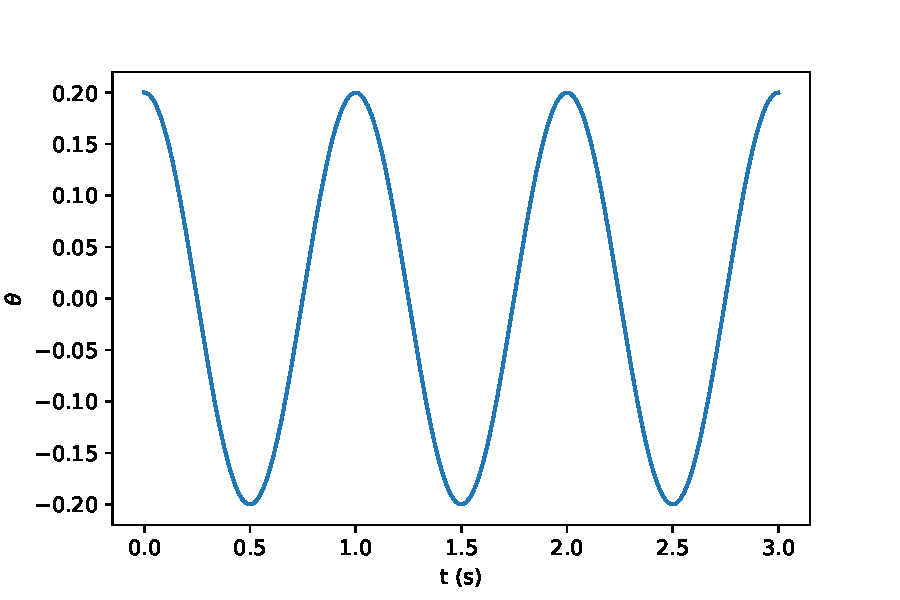
\includegraphics[height=0.33\textheight]{figs/pendulum/sho.pdf} 
\caption{The small angle approximation for pendulum motion with period $T_L=1~\rm s$}.
\label{fig:sho}
\end{center}
\end{figure}


Analytic solutions are the precious gems that we use to validate our
numerical techniques.  We'll start our analysis in a region where we
can solve the problem analytically.  For small displacements of the
pendulum, $\theta$ is small, and so:
\begin{displaymath}
\sin \theta \approx \theta
\end{displaymath}
and
\begin{displaymath}
\alpha = -\omega_L^2 \, \sin \theta \approx -\omega_L^2 \, \theta
\end{displaymath}
The differential equation which describes the motion is:
\begin{displaymath}
\frac{d^2\theta}{dt^2} = -\omega_L^2 \, \theta
\end{displaymath}
We showed in lecture that if the initial angular velocity is zero ($\omega_0 = 0$) and the initial theta position is $\theta_0$, then the solution is:
\begin{equation}
\label{eqn:sho}
\theta(t) = \theta_0 \cos(\omega_L \, t)
\end{equation}
as plotted in Fig.~\ref{fig:sho}.  The pendulum rocks back and forth
following a sine wave with period:
\begin{displaymath}
T_L = \frac{2 \pi}{ \omega_L} = 2 \pi \sqrt{\frac{L}{g}}
\end{displaymath}


\plot Calculate $\omega_L$ for a pendulum with $L=1~\rm m$ and $g=9.8~\rm m/s^2$.
What are the units of $\omega_L$?\\

\plot  Suppose you want to construct a pendulum such that for small
oscillations the period $T_L = 1~\rm s$.  What should be the value of
$\omega_L$?  What length $L$ should you use, assuming that $g=9.8~\rm
m/s$?\\

\newpage

\plot Reproduce the plot in Fig.~\ref{fig:sho}.  Set the
constants $T_L$, $\omega_L$, $\theta_0$, and $N$ as follows:
\begin{python}
TL = 1          # period in seconds 
wL = 2*np.pi/TL # small-angle angular frequency of pendulum 
A  = 0.2        # theta at t=0 (amplitude)
\end{python}
You must complete this problem {\bf without using an explicit for
  loop} and only {\bf six or less additional lines of code.}  (Debugging
print statements do not count toward this limit, use as many of those
as you like!)  To set the $y$ axis label to the fancy $\theta$ do:
\begin{python}
plt.ylabel("$\\theta$")
\end{python}.

\section{The Failure of the Euler Method}

The Euler equations for angle $\theta$ and angular velocity $\omega$ are:
\begin{eqnarray}
  \theta_{n+1} &=& \theta_n + \tau \, \omega \\
  \omega_{n+1} &=& \omega_n + \tau \, \alpha 
\end{eqnarray}
where $\alpha$ is the angular acceleration and $\tau$ is the time step.\\

\plot Implement a function
\begin{python}
def euler(tau, theta, omega, alpha):
   # your code here
   return theta, omega
\end{python}
which implements one iteration of the Euler method.
Test your \pyth{euler} function with these test values:
\begin{python}
print(np.around(euler(-0.01, -0.28, -0.30, -0.06),3))
print(np.around(euler( 0.94,  0.32, -0.85, -0.86),3))
print(np.around(euler( 0.92, -0.16,  0.38, -0.32),3))
print(np.around(euler( 0.31,  0.12, -0.91, -0.76),3))
print(np.around(euler(-0.14,  0.96,  0.66, -0.73),3))
\end{python}
which should produce the following output:
\begin{verbatim}
[-0.277 -0.299]
[-0.479 -1.658]
[0.19  0.086]
[-0.162 -1.146]
[0.868 0.762]
\end{verbatim}
You'll use this now thoroughly tested function more below.  Don't change it!\\

\plot  Apply the Euler method to the problem of small oscillations of a pendulum with $T_L=1~\rm s$ as in Fig.~\ref{fig:sho}.  First, set the parameters of your code just as before:
\begin{python}
TL = 1          # period in seconds 
wL = 2*np.pi/TL # small-angle angular frequency of pendulum 
A  = 0.2        # theta at t=0 (amplitude)
\end{python}
Then implement the Euler method as follows:
\begin{algorithm}
  $\theta$ := A
  $\omega$ := 0
  $\tau$ := 0.0003
  Create an empty array tjth which will contain $\theta$ positions of the trajectory
  Append $\theta$ to the array tjth.
  Repeat $N$ times:
     Calculate $\alpha = \omega_L^2 \theta$
     Update $\theta$ and $\omega$ for acceleration $\alpha$ and time step $\tau$ by calling euler().
     Append $\theta$ to the array tjth.
  Create an array t containting $N+1$ appropriately spaced time values.
  Plot tjth versus t
\end{algorithm} 
As always, first debug your code using a small value for $N$.  Then,
you should reproduce something that closely resembles Fig.~\ref{fig:sho} with
$N=10000$. \\

\plot Repeat the exercise above (you can use cut and paste) with $\tau=0.01$ and $N=1000$.  Yikes!  Is energy conserved?\\

\section{The Verlet Method}

The Verlet Equation for this problem is:
\begin{eqnarray}
  \theta_{n+1} &=& 2 \theta_n - \theta_{n-1} + \tau^2 \, \alpha
\end{eqnarray}
Notice that with the Verlet method, we will not need to calculate angular
velocity $\omega$ in order to get the $\theta$ trajectory.\\

\plot Implement a function
\begin{python}
def verlet(tau, theta, oldth, alpha):
   # your code here
   return theta
\end{python}
which returns $\theta_{n+1}$ from $\theta_n=$theta and
$\theta_{n-1}=$oldth using the verlet method.
Test your \pyth{verlet} function with these test values:
\begin{python}
print(np.around(verlet(-0.01, -0.28, -0.30, -0.06),3))
print(np.around(verlet( 0.94,  0.32, -0.85, -0.86),3))
print(np.around(verlet( 0.92, -0.16,  0.38, -0.32),3))
print(np.around(verlet( 0.31,  0.12, -0.91, -0.76),3))
print(np.around(verlet(-0.14,  0.96,  0.66, -0.73),3))
\end{python}
which should produce the following output:
\begin{verbatim}
-0.26
0.73
-0.971
1.077
1.246
\end{verbatim}
You'll use this now thoroughly tested function more below.  Don't change it!\\

\plot  In a previous exercise you showed that the Euler method, when applied to the problem of small oscillations of a pendulum with $T_L=1~\rm s$ for $\tau=0.01$ and $N=1000$, is unstable.  Instead, apply the Verlet method.  You can reuse (by copying and pasting) much of your code from that previous exercise with a few changes:
\begin{itemize}
 \item You will call your \pyth{verlet} function instead of \pyth{euler}.
 \item You no longer need to keep track of $\omega$ (\pyth{omega})
 \item You will now have to keep track of two $\theta$ values at all times.  At each updat:
\begin{displaymath}
   (\theta_n, \theta_{n-1}) \rightarrow  (\theta_{n+1}, \theta_{n})
\end{displaymath}
 \item You can start things off with \pyth{oldth = theta = A}
\end{itemize}
With this method, you should produce many oscillations with no sign of instability.\\

\plot So far, we have been using the small angle approximation.  Modify your code to use the exact formula for the angular acceleration $\alpha = \omega_L^2 \, \sin \theta$ and set the initial position to $A=2$.  This is a trivial change to your numerical simulation, but it  makes an analytic solution impossible!\\

\plot (Optional Challenge) Run you Verlet analysis for $N=1000$ steps
for $A=3$ and set $\tau$ appropriately so that you see a bit more than
one period of motion.  Plot the trajectory as a black line and read
off the period $T$.  Superimpose a plot of a cosine with amplitude $A$
and period $T$.\\

\plot (Optional Challenge) We've been starting things off with
approximately zero angular velocity by setting
\pyth{oldth = theta = A}.
You can add velocity to the initial state with:
\begin{python}
  V = 1
  theta = A
  oldth = A - tau*V
\end{python}
Give the pendulum enough of a whack that it reaches all the way to top
and keeps going.  When plotting this trajectory, you can use \pyth{np.mod} to
keep the theta values in the range from -$\pi$ to $\pi$ if you want.\\

\plot (Optional Challenge) Fix the Euler method for this pendulum
problem by forcing energy to be conserved at each step.  Compare your
results to the Verlet method.\\

















\chapter{Orbital Motion}

\section{Introduction}

\section{Orbital Motion}




\chapter{Integration}

\section{Introduction}

\section{Integration}

\section{Gaussian Distribution}

\section{Eliptic Function}




\chapter{The Monte Carlo Method}

\section{Introduction}

This lab, which will take two lab sessions to complete, introduces the
Monte Carlo method, an approach to solving a wide range of problems by
repeatedly drawing random numbers from a probability distribution.
You will produce a sequence of pseudorandom numbers.  You will use a
histogram to directly compare values of random variables to a
probability distribution function.  With these preliminaries in hand,
you will explore several widely used Monte Calro techniques: Monte
Carlo integration, the rejection method, and the transform method.
You will finish by looking at the evolution of entropy during
diffusion, as modeled by a random walk.

\section{Generating random numbers}

The Monte Carlo method relies on the generation of random numbers, so
we will start there.  The numbers we generate using computers are
actually ``pseudorandom'' numbers, because they are deterministically
obtained from an algorithm.  However, the algorithm is choosen so that
the numbers appear random for practical purposes.  This is no small
concern.  Much of the computational work in the early 1970's had to be
redone because of the widespread use of a deeply flawed pseudorandom
number generator called RANDU.

In this section, you will generate a pseudorandom number sequence
using the linear congruential method.  This sequence is determined
iteratively from the simple relationship:
\begin{displaymath}
  I_{n+1} = (a*I_{n} + c) \mod M
\end{displaymath}
Recall that $x \mod y$ (coded as {\tt x \% y} in python) is the remainder
after integer division $x//y$.  Each $I_n$ is called a seed, and the
initial seed $I_0$ must be provided e.g. by the user.  Notice that the
seeds are all integers in the range from 0 to $(M-1)$.  If we wish to
convert these seeds into a random variable $x$ in the range from 0 to
$L$, we simply use $x_n = L * I_n / M$.  As long as $M$ is much larger
than $L$, $x$ is approximately continous.

The algorithm works because the product $a*I_{n}$ is generally many
times larger than $M$, so the remainder is effectively a uniform
random number.  The effectiveness of this algorithm is highly
dependend on the choice of $a$,$c$, and $M$.  Choose poorly and you get
RANDU.  Choose wisely and you get the highly regarded algorithm of
Park and Miller.  We will do the latter and use $a=7^5$, $c=0$, and $M
= 2^{31}-1$.

\begin{samepage}
\begin{plot} \end{plot}
Generate a sequence of ten uniform random variables in the range
$[0,1]$ from the Park-Miller sequence, using an initial seed of one.
Check your code by testing that the generator returns a {\bf seed} of
1043618065 after 10000 calls.  Change the initial seed to a value of
your choice and report the first 10 random values.  If you like, round
to two decimal places using {\tt np.around} to tidy up your output.
\end{samepage}

\section{Visualizing distributions}

\begin{figure}[htbp]
 \begin{center}
 \begin{tabular}{cc}   
  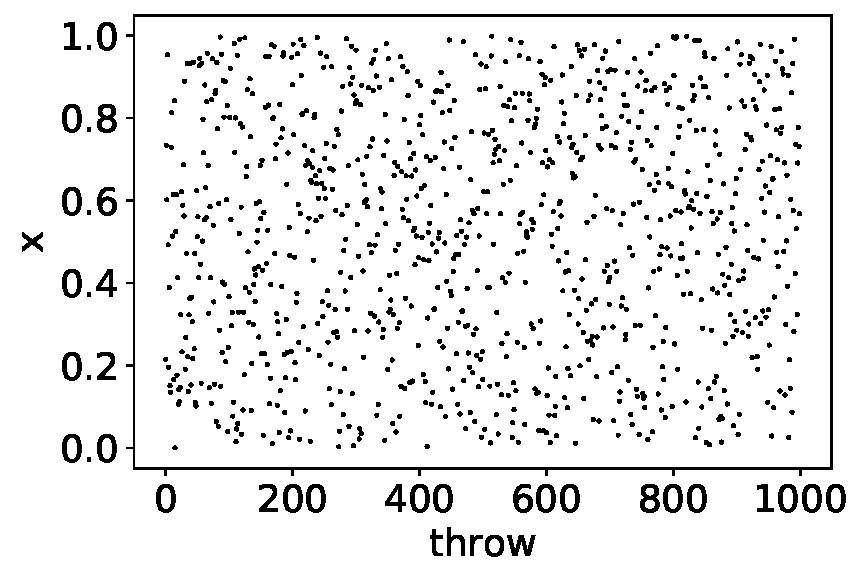
\includegraphics[height=0.22\textheight]{figs/labs/monte_carlo/flat2d.pdf} &
  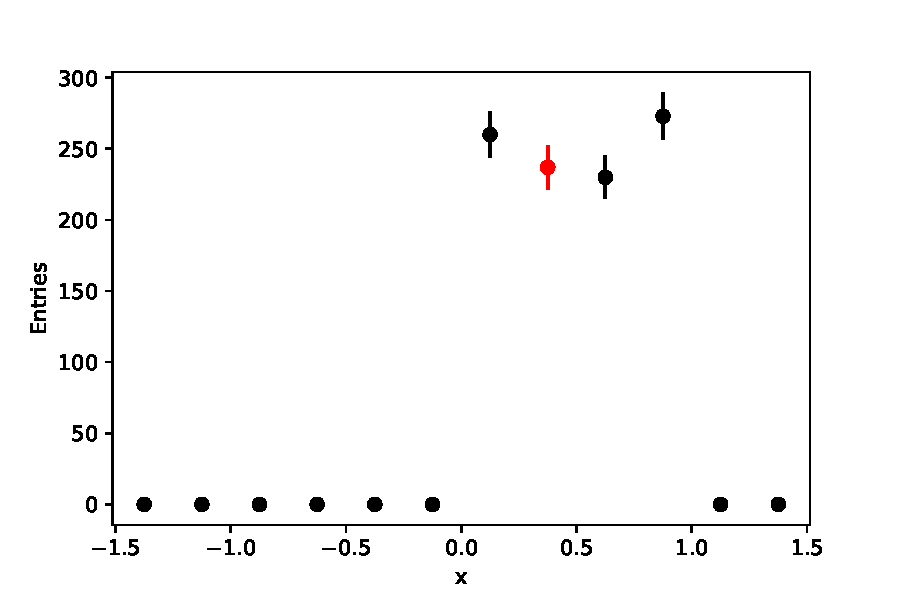
\includegraphics[height=0.22\textheight]{figs/labs/monte_carlo/flathist.pdf} \\
  (a) & (b) \\
 \end{tabular}
\caption{The (a) $x$ value of uniform random throws versus throw number and (b) corresponding histogram. }
\label{fig:flathist}
\end{center}
\end{figure}

\noindent
How can we verify that our Park-Miller random number generator
produces uniform random numbers in the range 0 to 1?  The associated
PDF is just $p(x)=1$, which we know how to plot, but how can we
compare this function to a sequence of numbers like $[0.21, 0.85,
  0.33, ...]$?  An initial attempt might look like
Fig.~\ref{fig:flathist}a, where we have simply plotted the $x$ value
of each throw versus the number of the throw.  Unfortunately, this
plot isn't particularly helpful.  If we zoomed in, we could determine
from the plot the $x$ value associated with each throw.  This is
simply too much information.

For interpreting a list of values as a distribution, there is only one
tool of choice: the histogram.  To histogram our data, we divide the
entire range $[0,1]$ into smaller ranges called {\em bins}.  Let's
start with 10 bins as an example. In this case, the first bin covers
the range from 0 to 0.1, or more precisely, the half-open interval
$\left[0,0.1\right)$ which includes $0$ and $0.099$, but not $0.1$.
  The second bin would have range $\left[0.1,0.2\right)$, the third
    bin would have range $\left[0.2,0.3\right)$ and so on, up to the
      last bin which would cover $\left[0.9,1.0\right]$.  To {\em
        fill} a histogram, you count the number of values that fall
      within the range of each bin.  So in our example, the value
      $0.21$ would add one to the count for the third bin, which has
      range $\left[0.2,0.3\right)$.  After filling, the histogram
        consists of a count associated with each bin range.

Fig.~\ref{fig:flathist}b shows a histogram filled with 1000 random
throws drawn from a uniform random number generator.  While we can now
see the shape of the distribution, we still don't have quite enough
information to answer the question, is this flat?  It is certainly not
perfectly flat!

The first feature we will need to add to the plot is the inclusion of
{\em error bars} to indicate the statistical uncertainty in our
histogram values.  Each histogram contains a {\em count} $n$ which
should follow a Poisson distribution with variance $\sigma^2 = n$.
Error bars are traditionally drawn with the size $\sigma$, which in
this case is $\sigma = \sqrt{n}$.  So when drawing a histogram, the
uncertainty in each bin is just the square root of the histogram
value.  That is the beauty of Poisson statistics!  If we have a count,
we know the statistical uncertainty.

\begin{figure}[htbp]
 \begin{center}
  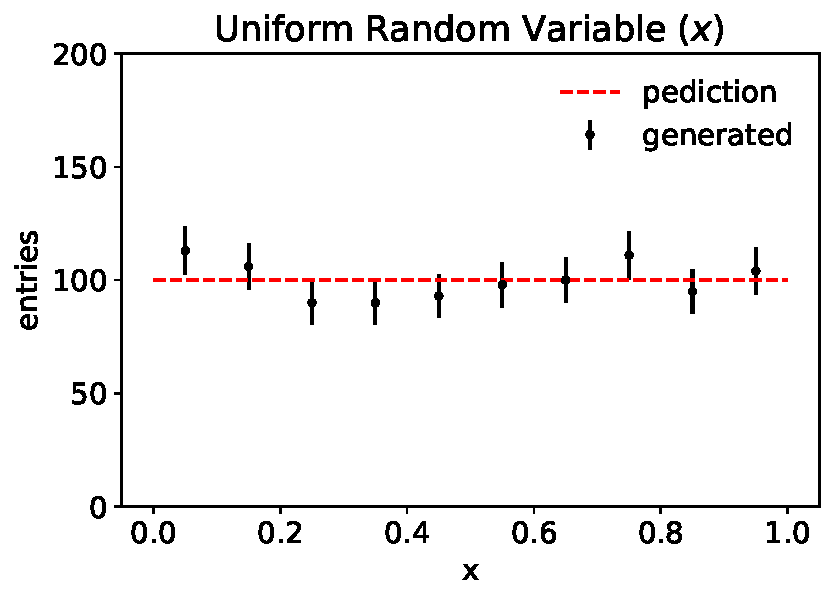
\includegraphics[width=0.50\textwidth]{figs/labs/monte_carlo/fancyhist.pdf}
  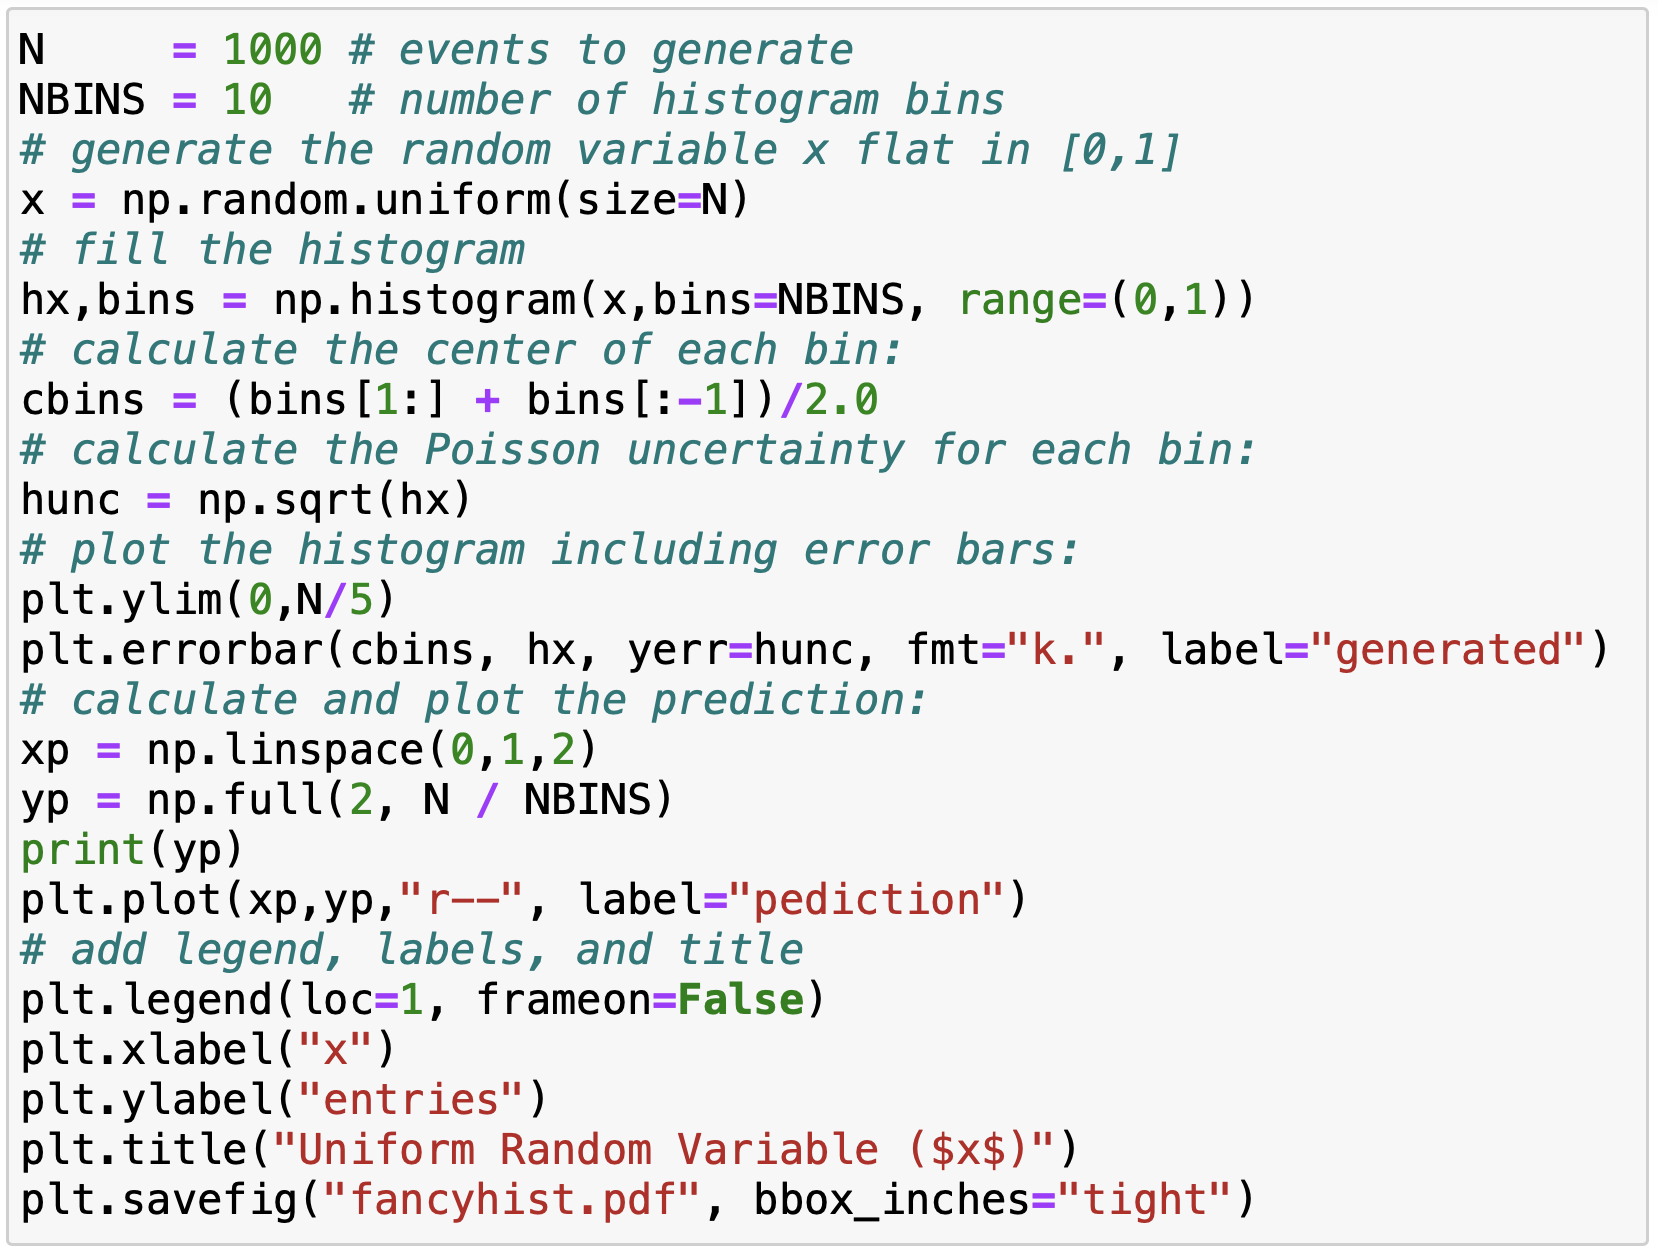
\includegraphics[width=0.75\textwidth]{figs/labs/monte_carlo/fancyhist-code.png}
\caption{Histogram of data drawn from a flat distribution compared to prediction, with the code used to produce the plot.}
\label{fig:fancyhist}
\end{center}
\end{figure}

We'll also want to add the prediction to the plot, assuming a flat
distribution for the contents of each bin.  In this case, we generated
$N$ events and we have $N_{\rm BINS}$ histogram bins, which should
therefore each contain an equal share: $N / N_{\rm BINS}$.  The
resulting histogram, along with the code used to generate it, is shown
in Fig.~\ref{fig:fancyhist}.  With the prediction and errorbars
included in the plot, one can now see that these generated values are
indeed quite consistent with a flat prediction. All of the bins are
within nearly one-sigma. With this number of bins, it is not uncommon
to see a two-sigma descrepancy.

You will produce many histograms in this class, so you will need to
(eventually) understand every single line in this example code.  Take
the time to read through the documentation for the key functions like
{\tt np.histogram} and {\tt np.random.uniform}, available on the web
(see numpy.org or just search ``np.histrogram python'').  A big part
of learning to program effectively, is learning how to read and
understand software documentation correctly and efficiently.

There are a few important features to notice:
\begin{itemize}
 \item The $x$-values are contained in an {\tt np.array} filled with
   uniform random variables generated by calling the {\tt
     np.random.uniform} function.
 \item The function {\tt np.histogram} is used to calculate a histogram
   from these $x$ values.  The call requests {\tt NBINS=10} histogram
   bins, in range $[0,1]$.  Don't confuse the python tuple {\tt (0,1)}
   used to indicate this range as indicating an open interval... often
   the computing language differs significantly from math notation, as
   is the case here!
 \item The {\tt np.histogram} function returns two items we need:  a {\tt np.array} containing the count for each bin ({\tt hx}) and a {\tt np.array} of bin edges ({\tt bins})
 \item We want to plot the count over the center of each bin, not one of the edges, so we calculate the quantity {\tt cbins} which is an {\tt np.array} containing the center of each bin.  You'll use this trick a lot, so make sure you understand what it is doing!
 \item The uncertainty on each bin {\tt hunc} is calculated as the square root of the bin counts {\tt hx}.
 \item We use the somewhat poorly named {\tt np.errorbar} function to plot {\bf both} the histogram central value {\tt and} the errorbar in each bin.
 \item We draw the prediction as a straight line defined by two points defined by {\tt xp} and {\tt yp}.
\end{itemize}

\begin{plot} \end{plot}
Modify the example code to generate a histogram for uniform random
numbers generated from your Park-Miller sequence instead of ${\tt
  np.random.uniform}$.  Increase the number of events to {\tt
  N=10000}.  Increase the number of bins to {\tt NBINS=20}.  Does your
code appear to produce uniform random numbers?

To answer a question in your notebook, simply add a cell and answer the question as a comment (each line starting with {\tt \#}).

\section{Calculating the value of $\pi$}

\begin{figure}[htbp]
\begin{center}
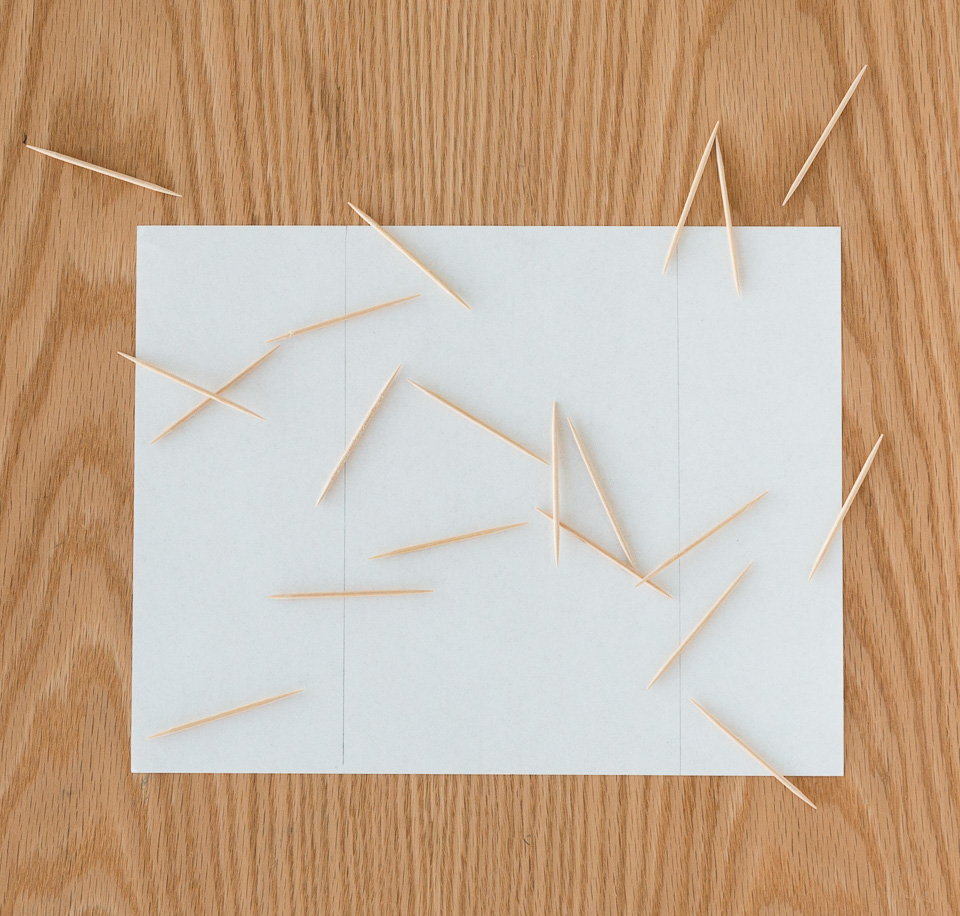
\includegraphics[width=0.65\textwidth]{figs/labs/monte_carlo/pitoss.jpg} 
\caption{Determining $\pi$ by throwing toothpicks.}
\label{fig:pitoss}
\end{center}
\end{figure}

\noindent
Hopefully 2021 will see the return of parties, so let's start by
examing a surefire way to be the life of the party: determining the
constant $\pi$ by throwing toothpicks!  The procedure is simple: you
cut a peice of paper to a width of four toothpicks, then draw two
vertical lines separated by the width of two tooth picks.  Take turns
tossing toothpicks, as in Fig.~\ref{fig:pitoss}.

From the geometry of the setup, it can be shown that the probability
that a toothpick which is entirely on the paper also crosses a line is
given by $1/\pi$.  Therefore, one can measure $\pi$ by counting the
total number of toothpicks that landed entirely on the page and
dividing by the number of those toothpicks that crossed a line.  This
is, in essence, the Monte Carlo method.

\begin{figure}[htbp]
\begin{center}
  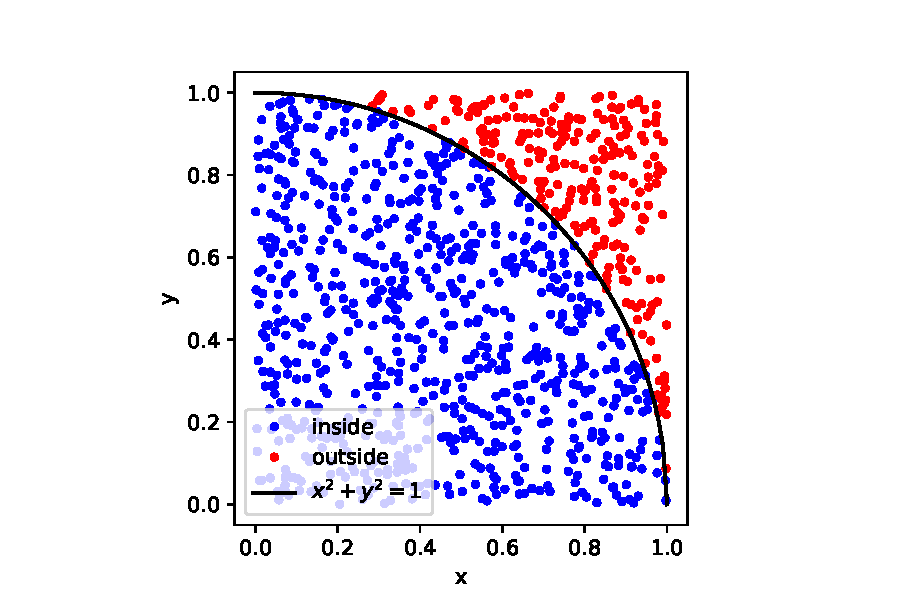
\includegraphics[width=0.50\textwidth]{figs/labs/monte_carlo/pimc.pdf}
  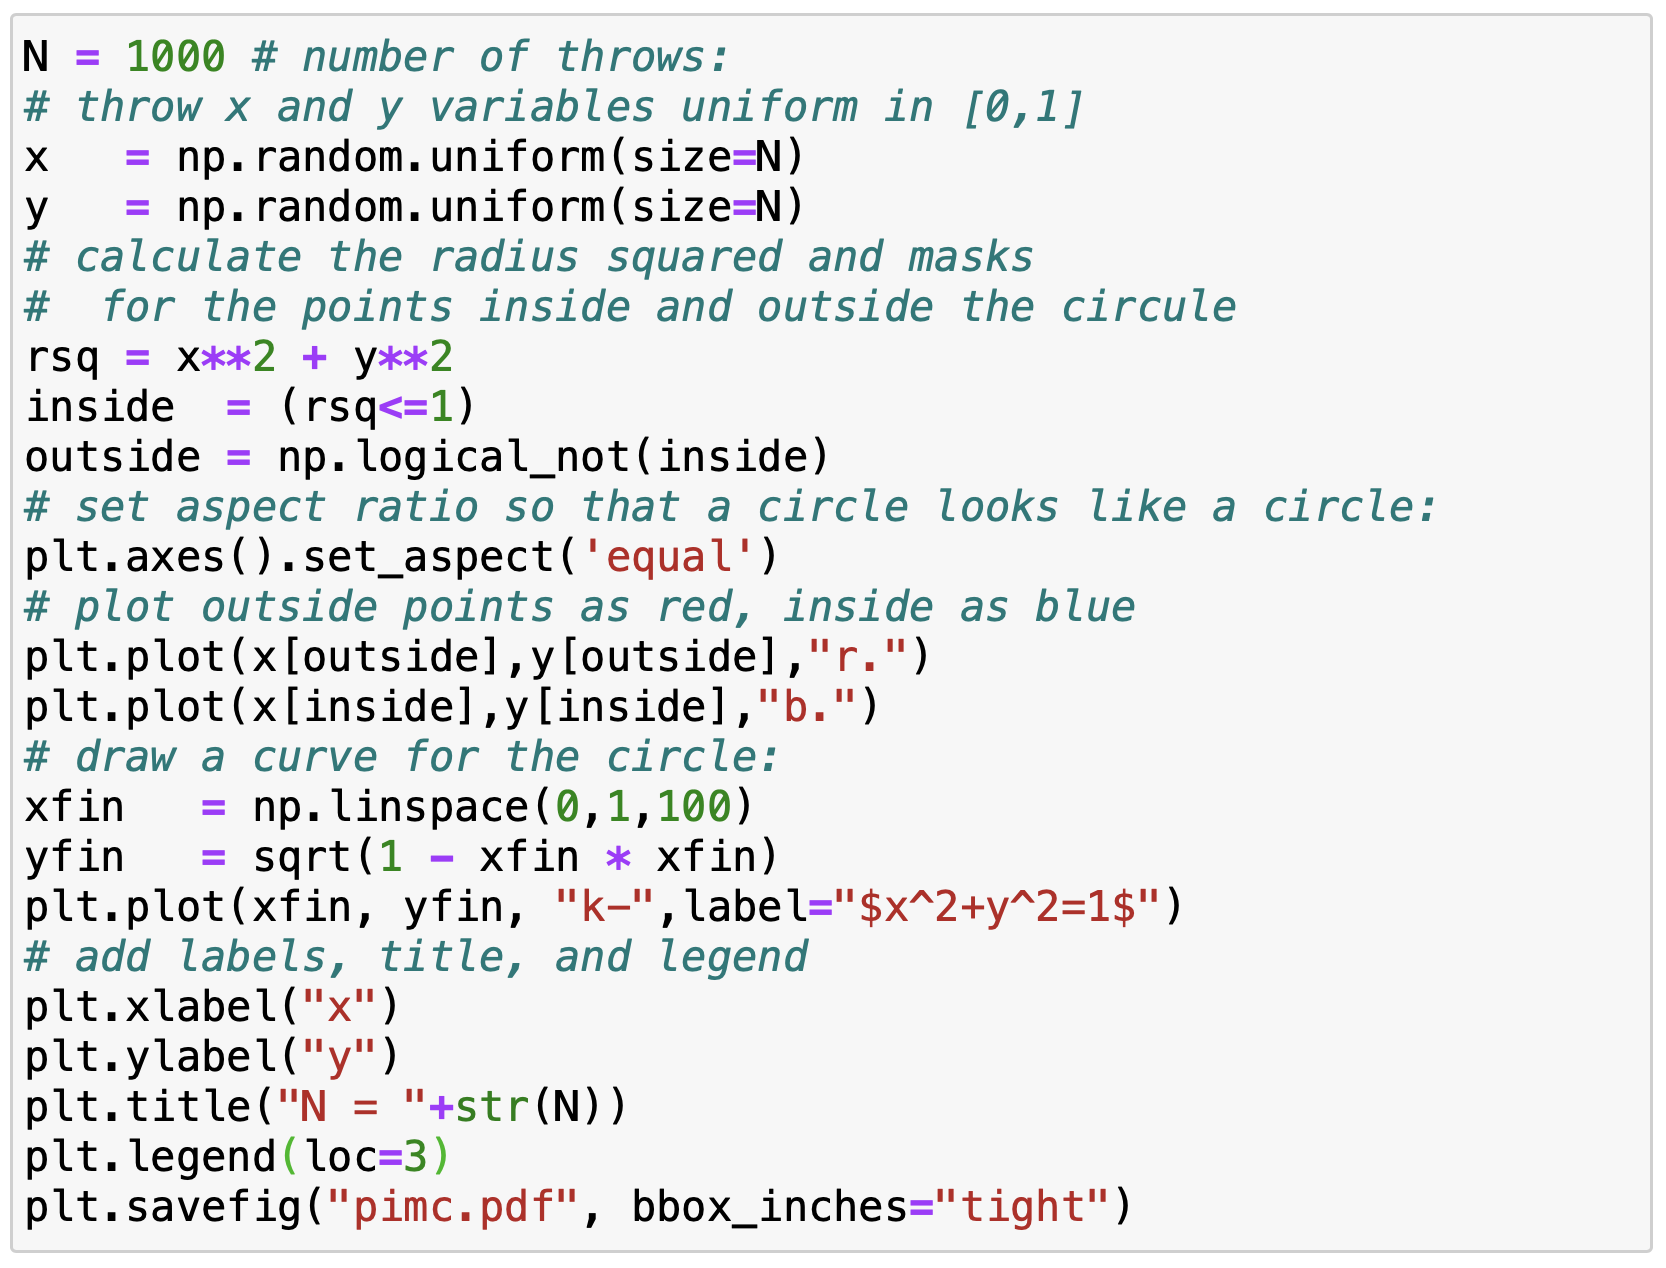
\includegraphics[width=0.75\textwidth]{figs/labs/monte_carlo/pimc-code.png} 
\caption{Monte Carlo Determination $\pi$ .}
\label{fig:pimc}
\end{center}
\end{figure}

An easier Monte Carlo method to implement computationally is shown in
Fig.~\ref{fig:pimc} along with the code used to generate the plot.
The idea is to throw points uniformly in the unit square of area 1.
Much like in the toothpick example, the value of $\pi$ can be
determined by counting the number of generated points that also landed
within the unit circle.

The key features of the example code are:
\begin{itemize}
\item The $x$ and $y$ values are each contained in an {\tt np.array} filled with uniform random variables in $[0,1]$ by the {\tt np.random.uniform} function.
\item A mask {\tt inside} is created to indicate which points are inside the circle.  Recall that the mask is an {\tt np.array} of True or False values, with the same length as the $x$ and $y$ arrays.  For example {\tt x[inside]} is an np.array containing just the subset of {\tt x} which are inside the circle.  
\end{itemize}

\begin{plot} \end{plot}
Starting from the example code, determine the numerical value of $\pi$
using the Monte Carlo method.  The easiest way to obtain the count you
need is to apply the function {\tt np.sum} to an appropriate mask.
When counting a mask, each True is treated as a one, and each False is
treated as zero.  Work out the relationship between $\pi$ and the
fraction of events in the unit circle, and use your count to
numerically determine the value of $\pi$.  Increase the number of
generated events and confirm that your calculated value of $\pi$
approaches the known value.

\begin{plot} \end{plot}
This is an example of a binomial process, because points are either
inside or outside the circle. So we expect the number of events in the
circle to follow the binomial distribution with $\sigma^2 = n \epsilon
(1-\epsilon)$.  In this case, $n$ is the total number of generated
events and $\epsilon$ is the fraction that fall inside the unit
circle.  The statistical uncertainty on your measured value of $\pi$
works out to be:
\begin{displaymath}
\sigma_\pi = \sqrt{\frac{\pi \, (4-\pi)}{n}}
\end{displaymath}
where $n$ is the number of generated events.  Does your measured value
of $\pi$ agree with the known value within your statistical
uncertainty?

\section{Monte Carlo integration}

The Monte Carlo method can also be used to numerically integrate a
function.  Monte Carlo integration methods generally only outperform
deterministic methods when the number of dimensions is large, but we
can illustrate the method most easily in one dimension. In this
section, you'll use the Monte Carlo method to perform the integral:
\begin{displaymath}
  \int_0^\pi \sin^2 \theta \, d\theta
\end{displaymath}

To do so, you should make a copy of your solution from the previous section
and modify it in the following manner:
\begin{itemize}
 \item Instead of thowing $x$ in $[0,1]$, throw $\theta$ in $[0,\pi]$.  This means the area of the rectangle $A$ is now $\pi$ instead of 1.
 \item Count the number of throws that land below the integral $y < \sin^2 \theta$.
 \item Determine the area under the curve as the fraction of the throws under the curve times the total area of the rectangle $A$.
 \item The statistical uncertainty in this case is $\pi/(2\sqrt{n})$ where $n$ is the number of generated events.
\end{itemize}  

\begin{plot} \end{plot}
Use the Monte Carlo method to calculate the integral:
\begin{displaymath}
  \int_0^\pi \sin^2 \theta \, d\theta
\end{displaymath}
Make a plot similar to that of Fig.~\ref{fig:pimc} showing the thows
above the curve in red and below the curve in blue.  Calculate the
integral and statistical uncertainty and compare it to the value you obtain analytically.

\section{The Rejection method}

\begin{figure}[htbp]
\begin{center}
  \begin{tabular}{cc}
  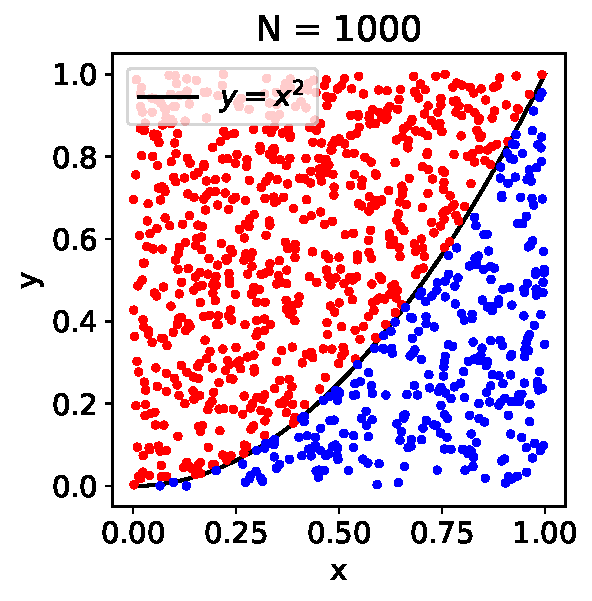
\includegraphics[height=0.30\textheight]{figs/labs/monte_carlo/rejectmc.pdf} &
  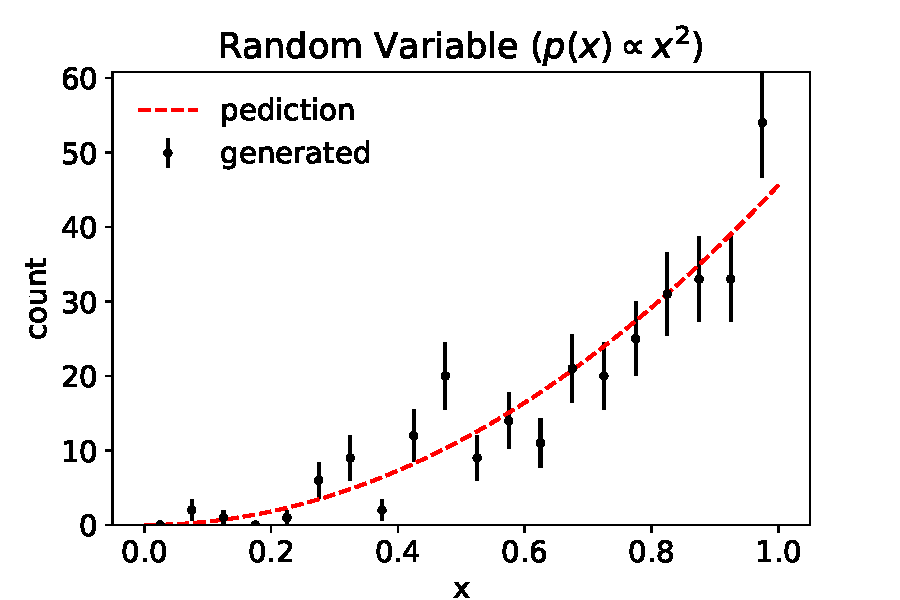
\includegraphics[height=0.30\textheight]{figs/labs/monte_carlo/quadhist.pdf} \\
  (a) & (b) \\
 \end{tabular}
  \caption{Monte Carlo rejection method applied to $p(x) \propto
    x^2$. Uniformly generated points (a) are rejected (red) if they
    are above the PDF, and the $x$ values of points below the PDF
    (blue) are selected.  A histogram (b) of the selected $x$ values
    shows that they follow the PDF.}
  \label{fig:rejectmc}
\end{center}
\end{figure}

\noindent
We now know how to generate uniform random numbers, but suppose we
need a random variable thrown according to a non-uniform probability
distribution $p(x)$?  Fig.~\ref{fig:rejectmc} demonstrates one
approach, which closely follows the procedure for numerical
integration using the Monte Carlo technique.

The rejection method produces random variables in a range from 0 to $L$
according to any desired PDF $p(x)$.  Start by finding a value $Y$ which is at
least as large as the maximum value of $p(x)$ for $x$ in $[0,L]$.  Then:
\begin{itemize}
  \item Throw $x$ as a uniform random variable in range $[0, L]$.
  \item Throw $y$ as a uniform random variable in range $[0, Y]$.
  \item If $y > p(x)$ reject the $x$ value and start over, otherwise, use the $x$ value as one throw.
\end{itemize}
Repeat these steps as necessary until a sufficent number of $x$ values have been selected.

The rejection method works because the probability of an $x$ value
being selected is, by construction, proportional to $p(x)$.  Since the
$x$ values were initially chosen from a flat distribution, the
selected $x$ values will follow the $p(x)$ distribution.  You can
visualize this in Fig.~\ref{fig:rejectmc} which leaves very little
doubt that the $x$ values of the blue points will follow the PDF.
Notice that it isn't even necessary for $p(x)$ to be normalized for
this procedure to work: any function proportional to the PDF of interest will do.

To produce a smooth function such as the quadratic prediction of
Fig.~\ref{fig:rejectmc}b, make sure you use plenty of $x$ values
(around 100 at least), via {\tt np.arange} or {\tt np.linspace}, just
as you did in the Plotting lab.  When comparing a PDF to histogrammed
data (as you will do for the second plot below) you will need to
normalize it appropriately.  The number of throws we expect to find in
a bin with edges at $a$ and $b$ is given by
\begin{displaymath}
  N \cdot \int_a^b p(x) \, dx \; = N \cdot p(x^*) \cdot (b-a) 
\end{displaymath}
The integral is simply the probability that one throw ends up in the
range, which we scale by the total number of throws $N$.  The equality
holds for at least one $x^*$ in the range $[a,b]$ and $(b-a)$ is
simply the bin size.  Therefore, we can formulate a prediction from a
normalized PDF $p(x)$ to data from $N$ throws used to fill a histogram with
bin sizes $\Delta x$ as the smooth function resulting from:
\begin{displaymath}
N \cdot p(x) \cdot \Delta x
\end{displaymath}
This is a technique we will use over and over again, so make sure you
understand it!

\begin{plot} \end{plot}
Use the rejection method to generate random numbers in the region from [0,1] that follow a distribution $p(x) \propto x^2$.  You'll do the following:
\begin{itemize}
  \item Note that there is no need to normalize the PDF when using the rejection method, so use $p(x)=x^2$.
  \item In our $x$ range $[0,1]$, $p(x)$ has maximum value at $x=1$ so set $Y = p(1) = 1^2 = 1$. 
  \item Throw $x$ as a uniform random variable in the range $[0, 1]$.
  \item As $Y=1$, throw $y$ as a uniform random variable in range $[0, 1]$.
  \item If $y > x^2$ reject the $x$ value and try a new set of $x$ and $y$ values, otherwise, use the $x$ value as one throw.
\end{itemize}
Throw 1000 (unselected) $x$ values, and produce a plot like that of
Fig.~\ref{fig:rejectmc}a showing your selected points in blue, your
rejected points in red, and the selection function ($p(x) = x^2$).

\begin{samepage}
\begin{plot} \end{plot}
Increase the number of (unselected) $x$ values thrown to 10,000.
Count the number $N$ of selected $x$ values.  Generate a plot like that of
Fig.~\ref{fig:rejectmc}b comparing the distribution of your selected
$x$ values to the prediction, which in this case is given by:
\begin{displaymath}
N \cdot 3x^2 \cdot \Delta x
\end{displaymath}
Be careful to use the number of selected $x$ values for $N$, not the total thrown (10000) before rejection.
\end{samepage}

\section{The transformation method}

Suppose that you need to throw random variables according to an
exponential distribution $p(x) = \exp(-x)$.  This PDF is defined for
$[0,+\infty)$ and properly normalized across this range as you can verify:
\begin{displaymath}
  \int_0^{+\infty} \exp(-x) \, dx = 1
\end{displaymath}    
The first problem is that we can only generate uniform random
variables up to a finite value $L$, not $+\infty$.  But let's suppose we are
willing to work aound this by simply cutting off the PDF at some large
value, like say we won't produce values with $x>100$.

With this change, the rejection method will work in principle.  But it
still has a major shortcoming.  Since $p(x)$ has a maximum value of 1,
and $x$ ranges from 0 to 100, the rectangle we will be filling with
uniform random points has area 100.  But our PDF, even when
integrated to $+\infty$, only has area 1.  So less than one out of
every 100 points we throw will be selected.  Perhaps we can live with
this, but then what if we need to go out to $x=1000000$.  Now only one
out of every million points will be selected.  In many scenarios, the
rejection method becomes too computationally inefficient to be of any
practical value.

In these case, we can use the transformation method instead of the
rejection method.  The transformation method is premised on the fact
that for {\em any} normalized PDF, we must have
\begin{displaymath}
  p(x) \geq 0
\end{displaymath}
everywhere and
\begin{displaymath}
  \int_{-\infty}^{+\infty} p(x) \; dx = 1
\end{displaymath}
as long as we take care to set $p(x)=0$ outside our range for $x$.  It follows from these properties that for any value of $y$ in the range $[0,1]$ there is a unique largest $x$ value for which:
\begin{equation} \label{eqn:mctransform}
  \int_{-\infty}^{x} p(x) \; dx = y
\end{equation}
From the fundamental theorem of calculus, we see that:
\begin{displaymath}
  dy = p(x) \, dx
\end{displaymath}
If the variables $y$ are drawn from a uniform distribution with PDF $q(y)=1$, then we see that:
\begin{displaymath}
 \int_{y_1}^{y_2} q(y) \, dy = \int_{x_1}^{x_2}p(x) \, dx.
\end{displaymath}
for $x_i$ and $y_i$ related by Eqn.~\ref{eqn:mctransform}.  This shows
that while $y$ is a uniform random variable ($q(y)=1$), the
corresponding $x$ values will distributed according to the desired PDF
$p(x)$.

That provides the mathematical justification for the transformation
method, which starts by finding the inverse function $f^{-1}(y)$ for:
\begin{displaymath}
  y = f(x) = \int_{-\infty}^{x} p(x) \, dx
\end{displaymath}
Then the procedure is:
\begin{itemize}  
 \item Throw $y$ as a uniform random variable in $[0,1]$.
 \item Find $x = f^{-1}(y)$
\end{itemize}
The $x$ values determined in this way will be drawn from the $p(x)$ distribution.  

There is an intuitive explanation for why this works.  The $y$ value is
essentially a fraction of the probability integrated by the PDF.  In a
region of $x$ where $p(x)$ is relatively large, the integral is
changing rapidly and so a large range of $y$ values map to this region
of $x$-values.  In a region of $x$ where $p(x)$ is relatively small,
the integral is not changing rapidly and so a small range of $y$
values map to this region of $x$-values.

Let's see how this applies to our exponential function.  In this case we calculate:
\begin{displaymath}
y = f(x) = \int_0^x \exp(-x) \, dx = 1 - \exp(-x)
\end{displaymath}  
which we invert to find:
\begin{displaymath}
x = - \ln(1-y)
\end{displaymath}  
To determine values of the random variable $x$, we follow this procedure:
\begin{itemize}
 \item Throw a $y$ value flat in [0,1]
 \item Caculate $x = -\ln(1-y)$
\end{itemize}
Repeat to produce as many $x$ values as needed.  Notice that this
procedure gives one usable $x$ value for every random throw.

\begin{plot} \end{plot}
Use the transformation method as described to generate 10,000 values
of a random variable thrown from an exponential function.  Produce a
plot like that of of Fig.~\ref{fig:rejectmc}b comparing the
distribution of your generated events to the prediction for $p(x) =
\exp(-x)$.  Remember to properly normalize your prediction based on
the bin size and number of events thrown.

\newpage
\section{Particle diffusion}

\begin{figure}[htbp]
\begin{center}
  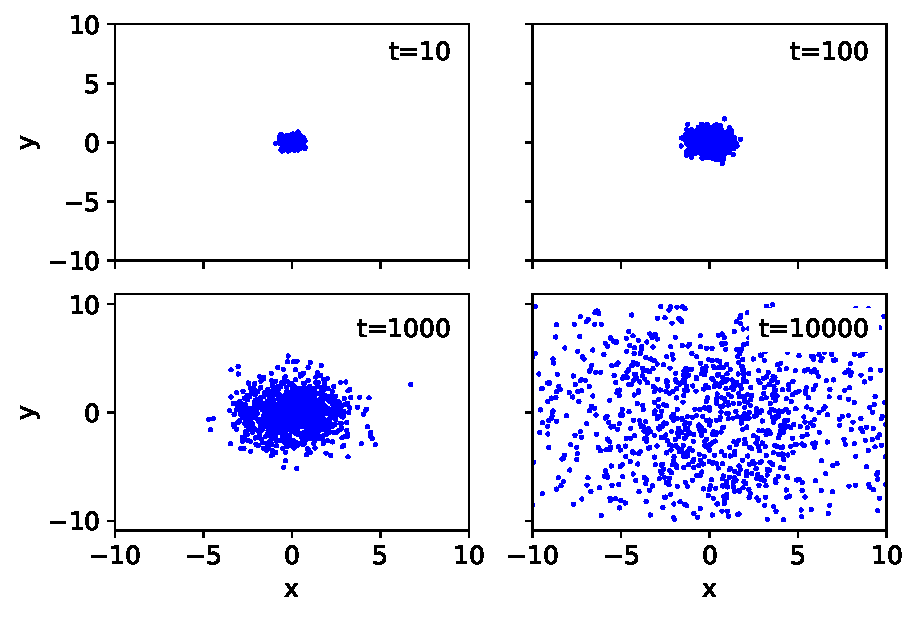
\includegraphics[width=0.80\textwidth]{figs/labs/monte_carlo/diffusion.pdf}
  \caption{Simulation of the diffusion of a drop of particles at four different times.}
\label{fig:diffusion}
\end{center}
\end{figure}

\begin{figure}[htbp]
 \begin{center}
  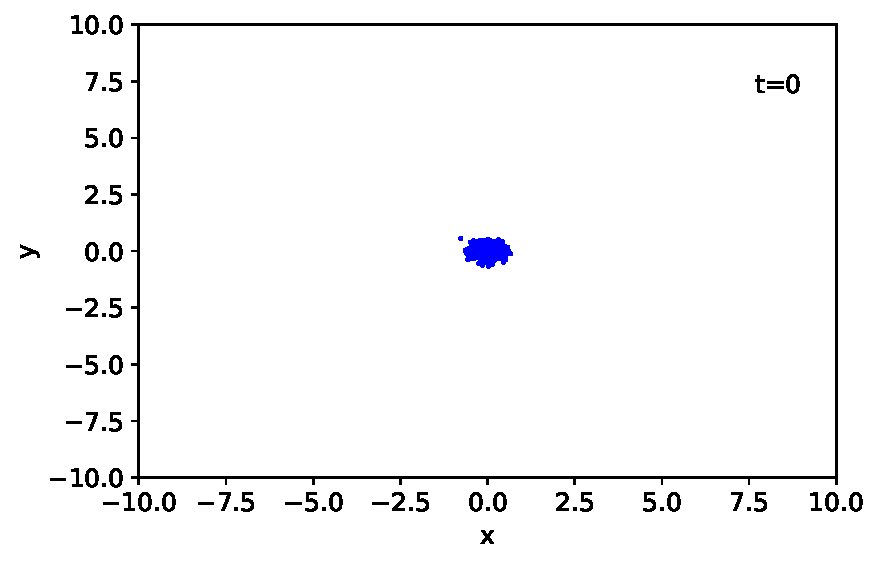
\includegraphics[width=0.50\textwidth]{figs/labs/monte_carlo/diffstart.pdf}
  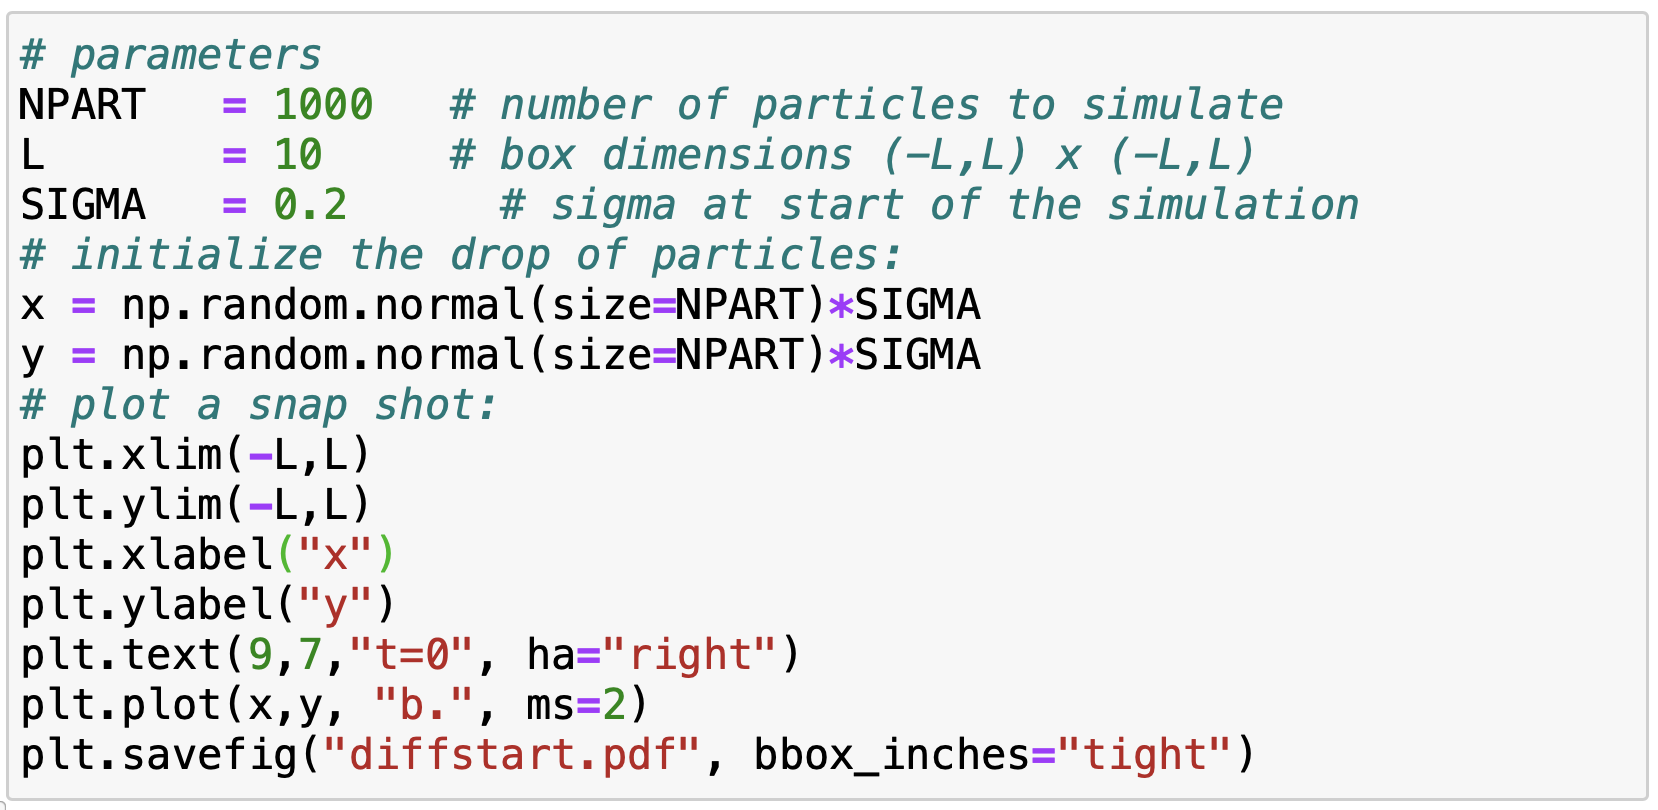
\includegraphics[width=0.75\textwidth]{figs/labs/monte_carlo/diffstart-code.png}
  \caption{Snapshot of the simulation at the start, along with the code used to produce it.}
\label{fig:diffstart}
\end{center}
\end{figure}


\noindent
In this section, we will model the diffusion of a drop of particles in
a medium, as in Fig.~\ref{fig:diffusion}, shown as snapshots at four
different times.  The starting point for the simulation, at $t=0$ is
shown in Fig.~\ref{fig:diffstart} along with the code used to produce
it.  The entire state of the system is contained in the arrays {\tt x}
and {\tt y} which contain the $x$ and $y$ positions of each particle.

The diffusion process is modeled by a random walk. During each update
(for one time step) the $x$ and $y$ values of each particle should be
randomly increased or decreased by an amount {\tt STEP=0.2} Any
particles that would leave the boundaries of the region $[-L,L]$ as a
result should be moved back into the region.  The numpy functions 
{\tt np.random.choice} and {\tt np.clip} are useful here.

Despite the symmetry of the random walk, the system clearly evolves by
diffusing outward over time.  This can be seen as a consequence of the
second law of thermodynamics.  Calculating the entropy from the
microscopic state of continuous particles is a bit tricky.  The
approach we will use is based on the Gibb's entropy.  We divide the
area into cells, and determine the fraction of the particles $f_i$ in
each cell $i$.  We calculate the entropy as:
\begin{displaymath}
  S = \sum_i f_i \ln f_i
\end{displaymath}
A python function which calculates the entropy in this manner:
\begin{tt}
\begin{verbatim}
from scipy import stats  
def entropy(x,y,l,sbins):
    h,xbins,ybins=np.histogram2d(x,y,bins=sbins,range=[[-l,l],[-l,l]])
    return stats.entropy(h.flatten())
\end{verbatim}
\end{tt}
The function takes as input parameters the position arrays {\tt x} and
{\tt y}, the boundary distance {\tt l} (set it to {\tt L} and the
number of bins in each dimension {\tt sbins} (set it to 20).  The
function returns the entropy of the current state of the system
described by {\tt x} and {\tt y}.

\begin{plot} \end{plot}
Starting from the example code, implement a random walk to model the
diffusion process, and plot four snap shops showing the evolution of
the system.

\begin{plot} \end{plot}
Calculate and record the entropy of the system as it evolves, and plot
the entropy as a function of time.



\chapter{Simulation of an Ideal Gas}

\section{Introduction}

For an ideal gas composed of molecules with mass $m$ at temperature
$T$, the probability density for the component of velocity in the $x$
direction ($v_x$) is given by:
\begin{equation}
  \label{eqn:mbvx}
P(v_x) = \sqrt{\frac{m}{2 \pi k_{\rm B} T}} \exp\left(-\frac{m v_x^2}{2k_{\rm B} T}\right)
\end{equation}
where $k_{\rm B}$ is Boltzmann's constant.  Similary for the $y$ direction:
\begin{equation}
  \label{eqn:mbvx}
P(v_y) = \sqrt{\frac{m}{2 \pi k_{\rm B} T}} \exp\left(-\frac{m v_y^2}{2k_{\rm B} T}\right).
\end{equation}

For simplicity, we will be simulating a gas in two dimensions.  The infinitesimal probability associated with a velocity $(v_x, v_y)$ is given by: 
\begin{eqnarray*}
P(v_x, v_y) \, dv_x \, dv_y &=& P(v_x) \, dv_x \, P(v_y) \, dv_y \\
   &=& \frac{m}{2 \pi k_{\rm B} T} \exp\left(-\frac{m (v_x^2+v_y^2)}{2k_{\rm B} T}\right) \, dv_x \, dv_y \\
   &=& \frac{m v}{2 \pi k_{\rm B} T} \exp\left(-\frac{m v^2}{2k_{\rm B} T}\right) \, d\theta \, dv \\
\end{eqnarray*}
where we have changed to polar coordinates $v$ and $\theta$ in the usual manner with area differential $dv_x \, dv_y = v \, dv \, d\theta$.  This allows us to read off the probability density in polar coordintes:
\begin{equation*}
P(v, \theta) = \frac{m v}{2 \pi k_{\rm B} T} \exp\left(-\frac{m v^2}{2k_{\rm B} T}\right) 
\end{equation*}
Integrating over all possible directions $\theta$, we obtain:
\begin{eqnarray}
P(v) &=& \int_0^{2\pi} P(v,\theta) d\theta \nonumber \\
     &=& \int_0^{2\pi} \frac{m v}{2 \pi k_{\rm B} T} \exp\left(-\frac{m v^2}{2k_{\rm B} T}\right) \nonumber \\
P(v) &=& \frac{m v}{k_{\rm B} T} \exp \left(-\frac{m v^2}{2k_{\rm B} T}\right) \label{eqn:mbv}\\
\nonumber
\end{eqnarray}
which is the Maxwell-Boltzmann distribution for an ideal gas in two
dimensions.  This is the probability density for a gas molecule to have speed
$v$.

In this lab, we will create a simple numerical simulation of an ideal
gas and verify that the velocity of the gas follows the
Maxwell-Boltzmann distribution.

\section{System of Units}

Choosing an effective system of units is essential for building a
well-behaved numerical simulation.  Consider the Maxwell-Boltzmann
distribution, which involves the following SI values:
\begin{itemize}
\item Boltzmann's constant: $k_{\rm B} = 1.38 \times 10^{-23}~\rm J/K$
\item Molecular masses: e.g. $N_2$ with $m =  4.65 \times 10^{-26}~ \rm kg$.
\item Temperature: e.g. room temperature $T = 293~\rm K$.
\end{itemize}
The smallest number greater than zero that a computer can represent
with a single-precision floating point number is approximately
$10^{-38}$. Representing the SI value of Boltzmann's constant at
$10^{-23}$ uses a large fraction of this precision before we even begin
our calculation.  Numerical algorithms using floating point numbers
work best when the values involved in the calculation are near one.

It is usually best, therefore, to devise an alternate system of units
for any numerical simulation which keeps the values of variables of
interest as near one as possible.  We will call this the numerical
system of units.

To start, we choose a reference temperature near the temperature
we would like to simluate, say $T_0 = 293~\rm K$.  All temperatures in
the simulation will be in units of this reference temperature.  So a
temperature {\tt T=1.2} in the program will be $1.2 \, T_0 = 352~\rm K$
in SI units.  Our model also includes mass, so we choose a reference
mass near the mass of the molecules we will be simulating, say $M_0 =
4.65 \times 10^{-26}~ \rm kg$.  A mass {\tt m=2.1} in our program would have
an SI value value of $2.1 M_0 = 9.8 \times 10^{-26}~ \rm kg$.

The physics we will simulate involves Boltzmann's constant $k_{\rm B}$
which will have a value of one in our program.  This sets the
reference energy from our reference temeperature.  For example, an
energy {\tt kT = 3} in our program will have an SI value of $k_{\rm B}
T = 3~k_B T_0 = 1.21 \times 10^{-20}~J$.  The reference energy and
reference mass together define a reference velocity:
\begin{displaymath}
V_0 = \sqrt{\frac{k_b T_0}{M_0}} = 295~ \rm m/s.  
\end{displaymath}  

The only time the actual values choosen for the numerical system of
units are needed is if you need to convert inputs in SI units to the
numerical system of units, or convert the results of your simulation
to SI units.  In this lab, we will specify all inputs and report all
results using the numerical system of units.  {\bf So there is no need for
specific values such as $M_0 = 2.32 \times 10^{-25}~\rm kg$ to appear
anywhere in your program.}  If such values do appear, outside of
comments, you are certainly making a mistake!

\begin{figure}[htbp]
\begin{center}
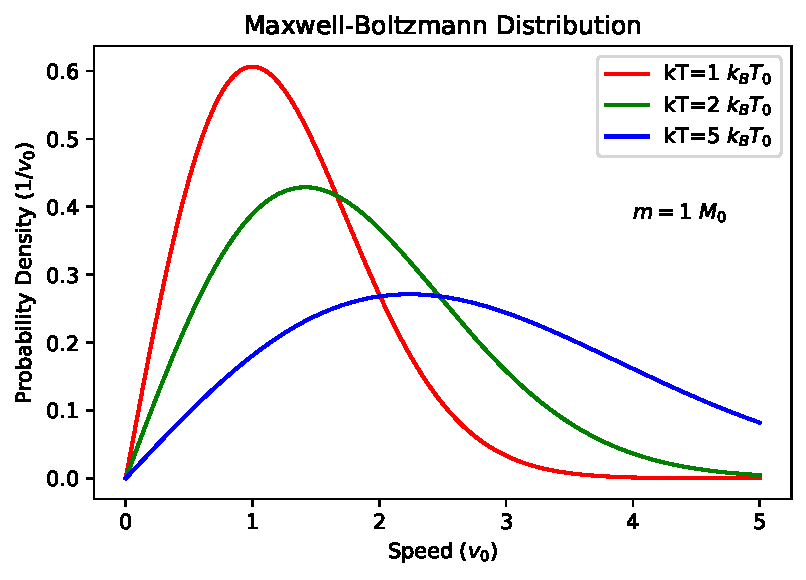
\includegraphics[width=0.65\textwidth]{figs/maxwellboltzman/maxboltz.pdf} \\
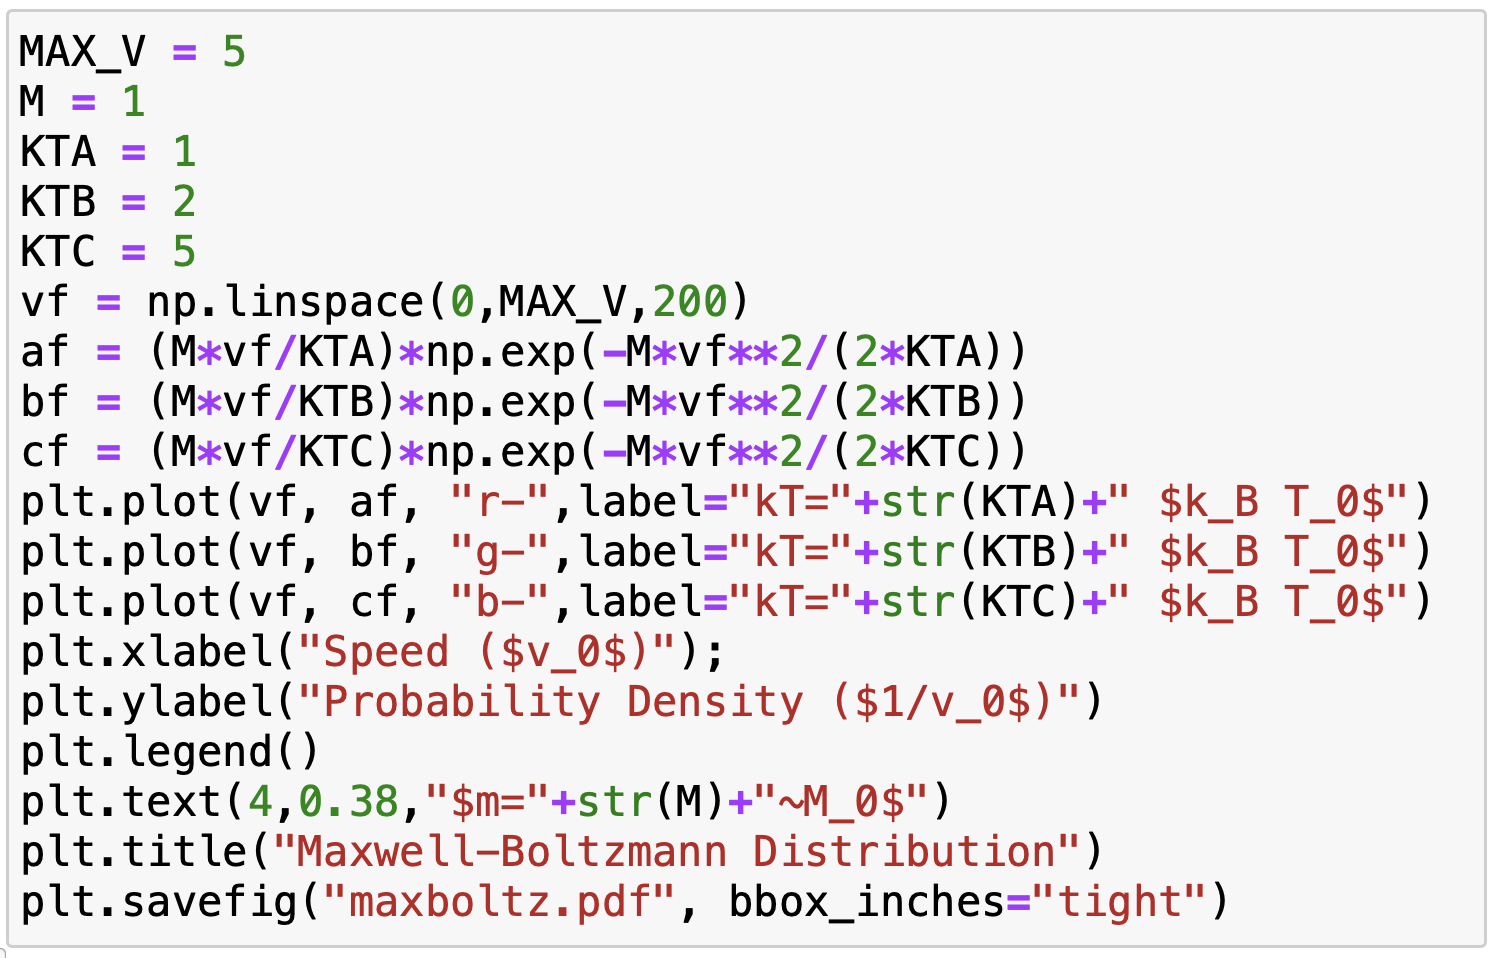
\includegraphics[width=0.65\textwidth]{figs/maxwellboltzman/maxboltz-code.png} \\
\caption{The Maxwell-Boltzmann distribution using a system of units appropriate for a numerical simulation, along with the code used to produce the plot.}
\label{fig:mbdist}
\end{center}
\end{figure}

As an example, the Maxwell-Boltzmann distribution is plotted in
Fig.~\ref{fig:mbdist} alongside the code used to produce it.  Notice
how for {\tt kT} and {\tt m} near one, the typical velcities are also
near one.  This is sign of good numerical system of units.  Notice
also that Boltzmann's constant or any other small or large numbers in
SI units do not appear anywhere in the code. 

\section{Collision Model}

At the heart of your numerical simulation is the collision model.  It
is the collisions of molecules that will allow your simulated gas to
reach thermal equilibrium.  We will use the simple elastic collision
of identical mass particles, as illustrated in Fig.~\ref{fig:collcms}, as our collision model.  We consider particles a and b with velocities $\vec{v_a}$ and
$\vec{v_b}$ in the lab frame.  The velocity of particle a in the CMS frame before the collision is
\begin{displaymath}
\vec{u} = \frac{\vec{v_a} - \vec{v_b}}{2}.
\end{displaymath}
The collision rotates the velocity of particle a by the scattering angle $\theta$ so that the velocity $\vec{w}$ after the collision is
\begin{displaymath}
\begin{pmatrix}
w_x \\
w_y \\
\end{pmatrix}
  =
\begin{pmatrix}
\cos \theta  & \sin \theta \\
-\sin \theta  & \cos \theta \\
\end{pmatrix}
\,
\begin{pmatrix}
u_x \\
u_y \\
\end{pmatrix}
\end{displaymath}
In the lab frame, the velocity of molecule a changes by an amount:
\begin{displaymath}
\Delta \vec{v_a} = \vec{w} - \vec{u}
\end{displaymath}
and the velocity of molecule b changes by an amount:
\begin{displaymath}
\Delta \vec{v_b} = \vec{u} - \vec{w}
\end{displaymath}




\begin{figure}[htbp]
\begin{center}
\begin{tikzpicture}
\draw[->, line width=1.5, blue] (-3,0) -- (-0.1,0);
\draw[->, line width=1.5, blue] (3,0)  -- (0.1,0);
\draw[->, line width=1.5, red] (0,0) -- (3*0.50,3*0.86) coordinate(A);
\draw[->, line width=1.5, red] (0,0) -- (-3*0.50,-3*0.86) coordinate(B);
\node[right] at (0.5,0.5) {$\theta$};
\node[left] at (-3,0) {a};
\node[right] at (3,0) {b};
\node[above] at (A) {a};
\node[below] at (B) {b};
\node[above] at (-1.5,0) {$\vec{u}$};
\node[above] at (1.5,0) {$-\vec{u}$};
\node[left] at (0.8,1.5) {$\vec{w}$};
\node[left] at (-0.8,-1.4) {$-\vec{w}$};
\end{tikzpicture}
\caption{The collision model in the center-of-mass:  incoming molecule $a$ with velocity $\vec{u}$ collides with the incoming particle $b$ of identical mass with velocity $-\vec{u}$.  Particle $a$ is scattered by angle $\theta$ and leaves with velocity $\vec{w}$, while particle $b$ leaves with velocity $\vec{w}$.  The magnitude of the final and initial velocities are the same:  $|\vec{u}| = |\vec{w}|$.}
\label{fig:collcms}
\end{center}
\end{figure}

\section{Implementing the Collision Model}

Our Python implementation for the collision will be computed in terms
of the components of the velocity vectors of molecule a and molecule
b:
\begin{eqnarray*}
\vec{v_a} &=& 
\begin{pmatrix}
a_x \\
a_y \\
\end{pmatrix} \\
\vec{v_b} &=& 
\begin{pmatrix}
b_x \\
b_y \\
\end{pmatrix} \\
\end{eqnarray*}
We'll use the Python variable names {\tt ax}, {\tt ay}, {\tt bx}, and {\tt by} to refer to $a_x$,  $a_y$,  $b_x$, and $b_y$.  

First calculate the $x$ and $y$ component of $\vec{u}$ as:
\begin{eqnarray*}
u_x &\equiv& \frac{a_x - b_x}{2} \\
u_y &\equiv& \frac{a_y - b_y}{2} \\
\end{eqnarray*}
Then compute the $x$ and $y$ component to the change in velocity of particle a and particle b:
\begin{eqnarray*}
  \Delta a_x &=& (\cos\theta - 1) \, u_x + \sin\theta \, u_y \\
  \Delta a_y &=& (\cos\theta - 1) \, u_y - \sin\theta \,  u_x \\
  \Delta b_x &=& (1-\cos\theta) \, u_x - \sin\theta \, u_y \\
  \Delta b_y &=& (1-\cos\theta) \, u_y + \sin\theta \,  u_x \\
\end{eqnarray*}
Finally, update the $x$ and $y$ components of the particle velocities to their value after the collision:
\begin{eqnarray*}
  a_x &\to& a_x + \Delta a_x \\
  a_y &\to& a_y + \Delta a_y \\
  b_x &\to& b_x + \Delta b_x \\
  b_y &\to& b_y + \Delta b_y \\
\end{eqnarray*}

In essential technique for programming complicated task is dividing
complicated tasks into smaller tasks, and thoroughly testing the
smaller tasks.  You cannot program effectively until you master this
technique.  I've taught students programming for many years, and the
students that finish last are invariably the ones that rush to
complete their entire program and then try to test and debug it.  This
approach always fails because when you do not get the right answer,
and you won't, ever, on the first try, you have absolutely no idea
what part of a very long chain of calculations is not programmed
correctly.

\begin{figure}[htbp]
\begin{center}
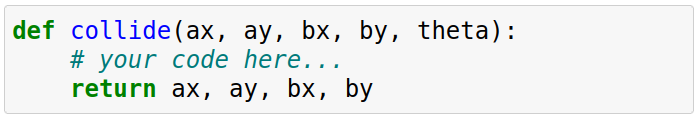
\includegraphics[width=0.65\textwidth]{figs/maxwellboltzman/collide.png} \\
\caption{Collision function.}
\label{fig:collfunc}
\end{center}
\end{figure}


To use this approach in the lab, we'll be implementing the collision
algorithm as a function, exactly as in Fig.~\ref{fig:collfunc}.  This
function takes as input the velocity components {\tt ax}, {\tt ay},
{\tt bx}, {\tt by} as defined above plus the scattering angle {\tt
  theta}.  In Fig.~\ref{fig:collfunc}, the function simply returns the
velocity components unchanged.  You should modify the function to
implement the scattering algoirthm described above.

Normally at this point, you would have to devise your own test to
validate your code.  One technique, that would work here, is to
calculate a few examples and then compare your program output to what
you obtained with paper and pencil.  For this lab, I will provide some
specific example calculations for you to validate your collision function.

\begin{figure}[htbp]
\begin{center}
  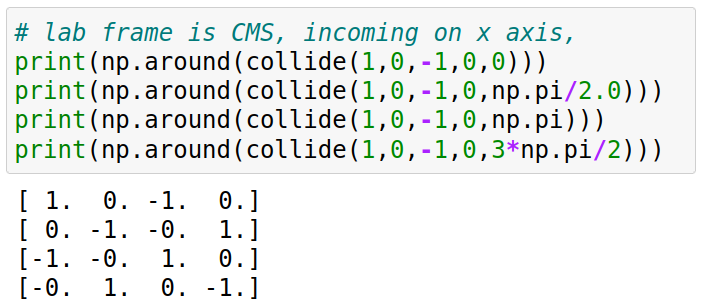
\includegraphics[width=0.65\textwidth]{figs/maxwellboltzman/collx.png} \\
  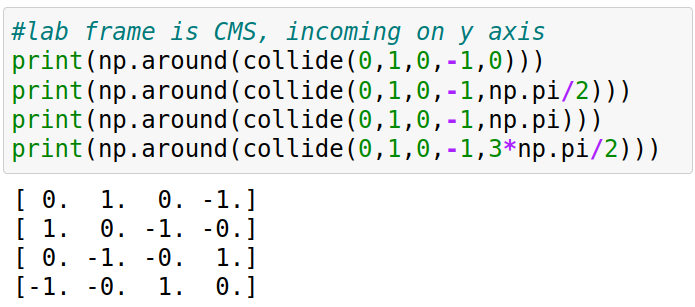
\includegraphics[width=0.65\textwidth]{figs/maxwellboltzman/colly.png} \\
  \caption{Example collisions along the $x$ and $y$ axis.}
\label{fig:collxy}
\end{center}
\end{figure}

\begin{plot} \end{plot}  Implement the collision algorithm as a function as in Fig.~\ref{fig:collfunc} and test it using example collisions from Fig.~\ref{fig:collxy}.

When testing your code, start with easy, special cases, such as used in Fig.~\ref{fig:collfunc}.  This helps makes it clearer where the program is failing.  Once your code works on the simple cases, escalate to more complicated examples.

\begin{figure}[htbp]
\begin{center}
  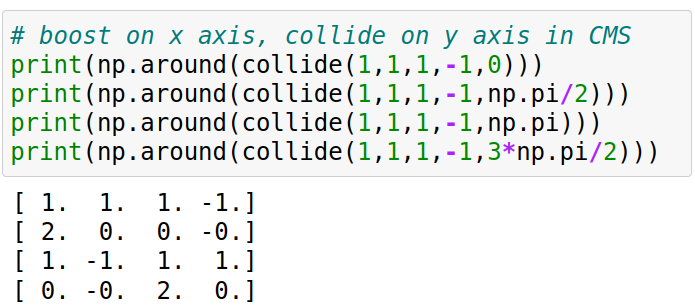
\includegraphics[width=0.65\textwidth]{figs/maxwellboltzman/collxy.png} \\
  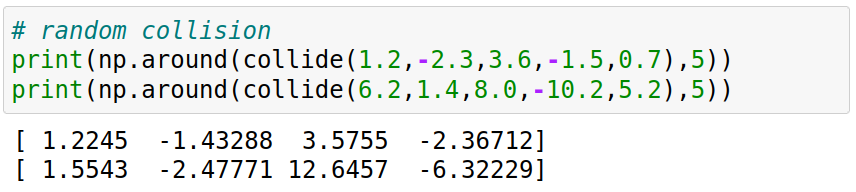
\includegraphics[width=0.65\textwidth]{figs/maxwellboltzman/collrand.png} \\
  \caption{More complicated example collisions.}
\label{fig:collcomp}
\end{center}
\end{figure}

\begin{plot} \end{plot}  Test your collision algorithm using the  example collisions from Fig.~\ref{fig:collcomp}.

\section{Initializing the Simulated Ideal Gas}

You will be modeling an ideal gas by direct Monte Carlo simulation of
{\tt NGAS} representative molecules.  We will use {\tt NGAS=1000}
intially, and you should use an even lower value while debugging.
We'll assume that the mass of each molecule in the gas is $M_0$,
or in the numerical system of units {\tt M=1}.

The state of your simulation will be completely contained in two numpy
arrays {\tt vx} and {\tt vy}, each of length {\tt NGAS}, which contain
the velocities of the particles in units of $V_0 = \sqrt{k_b T_0 /
  M_0}$.  Remember, the simulation uses a system of units that should
keep velocities near 1, so values such as 2.2, -3.1, 0.8, -0.01 are
all likely, and correspond to speeds up to several hundred meters per
second in SI units.  On the other hand, the presence of extremely
small values, like 5.3E-23, and extremely large values like 1.2E18 and
-8.2E28 are symptoms of bugs.

\begin{plot} Initialize both velocity arrays {\tt vx} and {\tt vy} of length {\tt NGAS}
with values choosen as uniform random variables in the range
$[-2,2]$. Fill two histograms, one with $v_x$ and one with $v_y$, with
an approriate range and 20 bins.  You should see that the velocities
are distributed uniformly (a flat distribution).  The distribution does not yet
resemble the Gaussian shape of Equation~\ref{eqn:mbvx} because it has not yet reached
thermal equilibrium.\end{plot}


\section{Collisions of an Ideal Gas}

To reach thermal equilibrium, you'll need to simulate collisions
betweens pairs of molecules in your gas.  For each collision, do the following:
\begin{itemize}
 \item Choose two molecules at random as particles $a$ and $b$. (See {\tt np.random.choice}.)
 \item Choose a random value $\theta$ uniformly in the range $[0,2\pi]$ (See {\tt np.random.uniform}.)
 \item Call your collision function with components of the velocity vectors for particles $a$ and $b$ and the scattering angle $\theta$.
 \item Update the velocity of particles $a$ and $b$ from the return value of your collision funciton
\end{itemize}   
For this model, you will need about 10 times as many collisions as gas
molecules in order to reach thermal equilibrium.

\begin{plot}  For {\tt NGAS=1000} simulate {\tt NCOLL = 10000} collisions as described above.
Fill two histograms, one with $v_x$ and one with $v_y$, with an
approriate range and 20 bins.  After reaching thermal equilibrium, the
distributions should resemble a Gaussian as predicted by Equation~\ref{eqn:mbvx}. \end{plot}

\section{Temperature of an Ideal Gas}

The temperature of the gas is related to the mean kinetic energy by:
\begin{equation}
\label{eqn:kt}
k_b T = m \, \frac{\braket{v_x^2} + \braket{v_y^2}}{2}  
\end{equation}  
You can estimate $\braket{v_x^2}$ from your simulation as {\tt np.mean(vx**2)}.

\begin{plot} Estimate $kT$ of the gas using Equation~\ref{eqn:kt} before and after simulating collisions.
The values should remain near the expected value 4/3.
\end{plot}

\section{The Maxwell-Boltzmann Distribution}

In this section, you'll reproduce the instructor plots of Fig.~\ref{fig:mbinst} using your own numerical simulation.

\begin{figure}[htbp]
\begin{center}
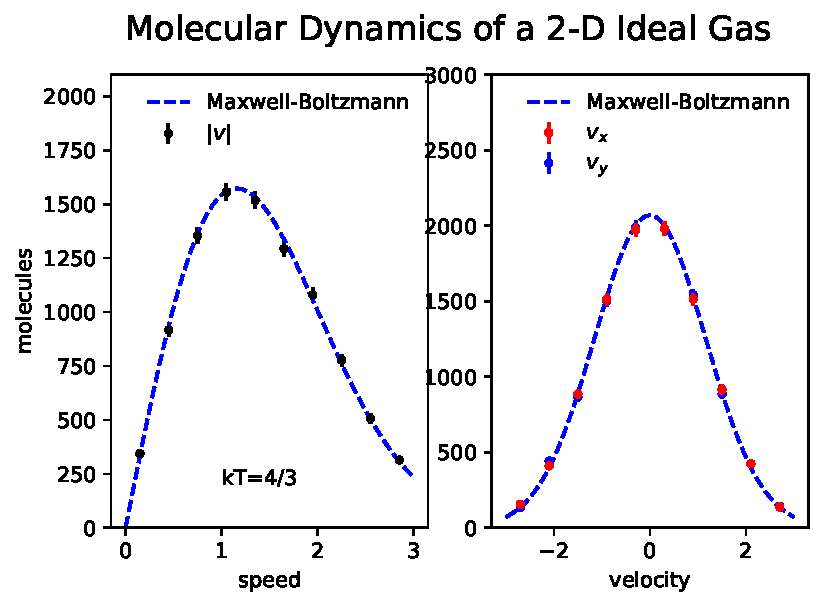
\includegraphics[width=0.85\textwidth]{figs/maxwellboltzman/maxboltz-instr.pdf} \\
\caption{Instructor plots.}
\label{fig:mbinst}
\end{center}
\end{figure}

\begin{plot}
  After your simulation reaches equilibrium, fill two histograms, one with $v_x$ and one with $v_y$, with an approriate range and 10 bins.  Compare with the prediction from Equation~\ref{eqn:mbvx}.  The results should resemble the right side of Fig.~\ref{fig:mbinst}, which were produced with {\tt NGAS=10000}.
\end{plot}

\begin{plot}
  After your simulation reaches equilibrium, fill a histograms with the magnitude of the velocity $v$, with an approriate range and 10 bins.  Compare with the prediction from Equation~\ref{eqn:mbv}.  The results should resemble the left side of Fig.~\ref{fig:mbinst}, which were produced with {\tt NGAS=10000}.
\end{plot}


  


\chapter{Vectors}

\section{Introduction}

In this lab, we will use numpy arrays to investigate the properties of
vectors in Euclidean space.

\section{Vector Dot Product and Cross Product }

In this lab, we will use numpy arrays of length 3 to represent vectors
in a Euclidean vector space.  So for example:
\begin{python}
  a = np.array([1.2, -3.2, 2.1])
\end{python}
is how we will represent the vector $\vec{a}$ with $a_x=1.2$,
$a_y=-3.2$, and $a_z=2.1$.  To obtain the components of the vector, we retrieve the appropriate element of the array, so $a_x$ is \pyth{a[0]},
$a_y$ is \pyth{a[1]}, and $a_z$ is \pyth{a[2]}.

We construct the unit vectors $\hat{x}$, $\hat{y}$ and $\hat{z}$ as:
\begin{python}
  xhat = np.array([1, 0, 0])
  yhat = np.array([0, 1, 0])
  zhat = np.array([0, 0, 1])
\end{python}
which provides an alternative way to define vectors:
\begin{displaymath}
\vec{b} = 2\hat{x} - 4\hat{y}+1\hat{z}
\end{displaymath}
using the equivalent python code:
\begin{python}
  b = 2*xhat - 4*yhat + 1*zhat
\end{python}

The dot product of two vectors is defined as:
\begin{displaymath}
\vec{a}\cdot\vec{b} = a_x \, b_x +  a_y \, b_y +  a_z \, b_z.
\end{displaymath}
We can determine the magnitude of vector using the dot product:
\begin{displaymath}
  |\vec{a}| = \sqrt{\vec{a}\cdot\vec{a}}
\end{displaymath}
The cross product of two vectors is defined as:
\begin{displaymath}
  \vec{a}\times\vec{b} =
  (a_y \, b_z -  a_z \, b_y) \; \hat{x}
  + (a_z \, b_x -  a_x \, b_z) \; \hat{y}
  + (a_x \, b_y -  a_y \, b_x) \; \hat{z}
\end{displaymath}

\vskip 0.25cm
\plot Implement a function \pyth{dot(a,b)} which returns the dot product of vectors a and b.  You do not need to use a for loop in your implementation if you do not want to: explicitly calling each of three components is simple and clear.  Confirm that your code is working by calculating $\vec{b}\cdot\hat{x}$, $\vec{b}\cdot\hat{y}$, and $\vec{b}\cdot\hat{z}$. \\


\plot Implement a function \pyth{mag(a)} which returns the magnitude of the vector a by calling your \pyth{dot(a,b)} function.  Show that your function works by comparing the magnitude of $\vec{b}$ return by your function with what you expect from paper and pencil.\\

\plot Implement a function \pyth{cross(a,b)} which returns the cross products of the vectors a and b.  Show that your function works for:
\begin{eqnarray*}
  \hat{x} \times \hat{x} &=& 0\\    
  \hat{x} \times \hat{y} &=& \hat{z}\\
  \hat{x} \times \hat{z} &=& -\hat{y}\\
  \hat{y} \times \hat{x} &=& -\hat{z}\\
  \hat{y} \times \hat{z} &=& \hat{x} \\ 
\end{eqnarray*}


The follow example demonstrates that:
\begin{displaymath}
\vec{a} \cdot \vec{b} \leq |\vec{a}|\,|\vec{b}|
\end{displaymath}
by generating many random vectors and testing:
\begin{python}
TOL = 10*np.finfo(float).eps
fail = 0
for i in range(10000):
    ra = np.random.rand(3)
    rb = np.random.rand(3)
    x = dot(ra,rb)-mag(ra)*mag(rb)
    if (x>TOL):
        fail = fail+1
print("failures:  ", fail)
\end{python}
Notice the use of a tolerance instead of strict comparison with zero
to account for the floating point precision.\\

\begin{plot} Demonstrate\end{plot}
\begin{displaymath}
  |\vec{a} + \vec{b}| < |\vec{a}| + |\vec{b}|
\end{displaymath}

\vskip 0.25cm
\begin{plot} Demonstrate the Jacobi identity:\end{plot}
\begin{displaymath}
 \vec{a} \times (\vec{b} \times \vec{c}) + \vec{b} \times (\vec{c} \times \vec{a}) + \vec{c} \times (\vec{a} \times \vec{b}) = 0
\end{displaymath}

\section{Numpy Tools}

The numpy tools for dot and cross products are \pyth{np.dot} and \pyth{np.cross}
\begin{python}
print(np.dot([1,2,3],[0,0,1]))
print(np.cross([1,0,0],[0,1,0]))
\end{python}

\section{Motion of a Charged Particle in a Magnetic Field}



\chapter{Matrices, Rotations and Parity}

\section{Introduction}

\section{Preparation}

\section{Rotations and Parity}
\begin{python}
def rotz(theta):
    cs = np.cos(theta)
    sn = np.sin(theta)
    R  = np.array([[cs, sn, 0],[-sn, cs, 0], [0, 0, 1]])
    R=np.around(R,decimals=15)+0
    return R
\end{python}

\begin{plot} With $\tau \equiv 2 \pi$ print the rotation matrix for $\theta = 0, \tau/4, \tau/2, 3 \tau/4, \tau$\
 corresponding to zero, quarter turn, half turn, 3/4 turn, and a full turn.\end{plot}



\begin{plot} Show that $R(\vec{a} \times \vec{b}) = (R\vec{a}) \times (R\vec{a})$.\end{plot}


\begin{plot} Show that $P(\vec{a} \times \vec{b}) \neq (P\vec{a}) \times (P\vec{a})$.\end{plot}



\chapter{Potential Energy and Symmetry}

\section{Introduction}

\section{Integration}




\chapter{Scattering}

\section{Introduction}

\section{Scattering}




\chapter{Roots}

\section{Introduction}

\section{Roots}

\section{Projectile Motion}

\section{Particle in a Box}

\section{Turning Points in Gravitational Motion}




\chapter{Linear Algebra}

\section{Introduction}





%\appendix

\chapter{Debugging}

In our context, debugging is the process of finding and removing
mistakes, called bugs, from your software.  Singling this process out
is a bit deceptive, it makes it seems distinct from software
development, as if you should write your software, and then debug it.
Indeed many students start this way, but it is a painful and
ineffective approach.  Experienced programs debug {\em while} developing
their code.

The fundamental approach to debugging (which works equally well
outside of programming) is to break every problem down into simple,
well defined parts, and then thoroughly test each part.  When one part
does not work, you break it down into smaller parts.  This process can
be quite simple, such as adding print statements to each step of a
complicated calculation.  It can also be quite advanced, such as when
teams of experienced software developers use automated builds and a
suite of integration tests that validate every proposed change to code
before it is accepted.  Experienced programs still produce bugs, they
just get better at squashing them.

There are a number of well-loved techniques to debugging:
\begin{itemize}
\item Print statements.
\item Start with a simple problem.
\item Test on special cases.
\item Use paper and pencil.
\item Decrease the size.
\item Establish feedback.
\item Write modular code.
\item Maintain unit tests.
\end{itemize}


\end{document}


